%==============================================================================
%  Especificación de Requisitos de Software (SRS), versión 1.2
%  Plataforma para la Gestión de Desastres y Reconstrucción
%  Arquitectura de Software, Pontificia Universidad Javeriana
%  Archivo autocontenido: pegar como main.tex en Overleaf (pdfLaTeX).
%  Figura requerida junto a este archivo: contexto.pdf
%==============================================================================
\documentclass[11pt,letterpaper]{article}

\usepackage[utf8]{inputenc}
\usepackage[T1]{fontenc}
\usepackage{lmodern}
\usepackage[spanish,es-tabla]{babel}
\usepackage[margin=2.4cm,top=2.6cm,bottom=2.6cm]{geometry}
\usepackage{graphicx}
\usepackage{booktabs}
\usepackage{longtable}
\usepackage{tabularx}
\usepackage{array}
\usepackage{xcolor}
\usepackage{csquotes}
\usepackage{pdflscape}
\usepackage{caption}
\usepackage{float}
\usepackage{enumitem}
\usepackage{siunitx}
\usepackage{ragged2e}
\usepackage{fancyhdr}
\usepackage[hidelinks]{hyperref}
\usepackage[spanish,nameinlink]{cleveref}

\hypersetup{
  pdftitle={Especificación de Requisitos de Software. Plataforma para la Gestión de Desastres y Reconstrucción},
  pdfauthor={Samuel Gantiva; Daniel Guiza; Juan Rubiano},
  pdfsubject={Arquitectura de Software. Proyecto del semestre, entrega 2}
}

%------------------------------------------------------------------ formato ---
\sisetup{
  output-decimal-marker={,},
  group-minimum-digits=5,
  group-separator={\,},
  mode=text,
  reset-text-series=false,
  text-series-to-math=true,
  reset-text-shape=false
}

% Se conserva la denominación "Cuadro" que usan los tres documentos del proyecto.
\addto\captionsspanish{%
  \renewcommand{\tablename}{Cuadro}%
  \renewcommand{\listtablename}{Índice de cuadros}}
\crefname{table}{Cuadro}{Cuadros}
\Crefname{table}{Cuadro}{Cuadros}
\crefname{figure}{Figura}{Figuras}
\Crefname{figure}{Figura}{Figuras}
\crefname{section}{sección}{secciones}
\Crefname{section}{Sección}{Secciones}
\crefname{subsection}{sección}{secciones}
\Crefname{subsection}{Sección}{Secciones}
\crefname{subsubsection}{sección}{secciones}
\Crefname{subsubsection}{Sección}{Secciones}

\setlength{\parskip}{0.45em}
\setlength{\parindent}{0pt}
\renewcommand{\arraystretch}{1.25}
\setlength{\tabcolsep}{4pt}
\setlength{\LTleft}{0pt}
\setlength{\LTright}{\fill}
\tolerance=1500
\emergencystretch=3em
\captionsetup{font=small,labelfont=bf}
\setlist{itemsep=1pt,topsep=3pt,parsep=0pt}

\pagestyle{fancy}
\fancyhf{}
\fancyhead[L]{\footnotesize SRS. Plataforma para la Gestión de Desastres y Reconstrucción}
\fancyhead[R]{\footnotesize\thepage}
\renewcommand{\headrulewidth}{0.4pt}
\setlength{\headheight}{14pt}
\fancypagestyle{plain}{\fancyhf{}\renewcommand{\headrulewidth}{0pt}}

\newcolumntype{L}[1]{>{\RaggedRight\arraybackslash}p{#1}}
\newcolumntype{C}[1]{>{\Centering\arraybackslash}p{#1}}

% Marcas: requisito o actor derivado, e inferencia del equipo
\newcommand{\derivado}{\textsuperscript{\textdagger}}
\newcommand{\inferencia}{\textsuperscript{\textasteriskcentered}}
\newcommand{\prim}{\newline (P)}

% Encabezado repetido de un cuadro largo:
% \cabecera{columnas}{etiqueta}{título}{fila de encabezado}
\newcommand{\cabecera}[4]{%
  \caption{#3}\label{#2}\\
  \toprule #4 \\ \midrule
  \endfirsthead
  \multicolumn{#1}{@{}l}{\small\itshape (continuación del \cref{#2})}\\
  \toprule #4 \\ \midrule
  \endhead
  \bottomrule
  \endfoot}

% Ficha de un escenario de atributo de calidad: \fichaqa{etiqueta}{título}
\newcommand{\fichaqa}[2]{%
  \caption{#2}\label{#1}\\
  \toprule \textbf{Parte} & \textbf{Contenido} \\ \midrule
  \endfirsthead
  \multicolumn{2}{@{}l}{\small\itshape (continuación del \cref{#1})}\\
  \toprule \textbf{Parte} & \textbf{Contenido} \\ \midrule
  \endhead
  \bottomrule
  \endfoot}

%==============================================================================
\begin{document}

\begin{titlepage}
\centering
\vspace*{2.2cm}
{\large Pontificia Universidad Javeriana\\ Facultad de Ingeniería\\ Departamento de Ingeniería de Sistemas\par}
\vspace{0.4cm}
{\large Arquitectura de Software\par}
\vspace{2.2cm}
{\Huge\bfseries Especificación de Requisitos\\[3mm] de Software (SRS)\par}
\vspace{1.0cm}
{\LARGE Plataforma para la Gestión\\[2mm] de Desastres y Reconstrucción\par}
\vspace{1.6cm}
{\large\itshape Entrega 2\par}
{\large Requisitos funcionales, atributos de calidad,\\ análisis de una solución existente y diagrama de contexto\par}
\vspace{2.2cm}
{\large Samuel Gantiva \quad$\cdot$\quad Daniel Guiza \quad$\cdot$\quad Juan Rubiano\par}
\vspace{1.2cm}
{\large 18 de noviembre de 2026\par}
\vfill
{\small Versión 1.2\par}
\end{titlepage}

\section*{Control de cambios}

\noindent\begin{tabular}{L{1.5cm} L{3.2cm} L{11.0cm}}
\toprule
\textbf{Versión} & \textbf{Fecha} & \textbf{Cambios} \\
\midrule
1.0 & 24 de septiembre de 2026 & Versión entregada. \\
1.1 & 9 de noviembre de 2026 & Se atienden las observaciones del profesor sobre la versión 1.0.
Se corrige el diagrama de contexto (dirección y etiqueta de cada flujo).
Se completan los actores y se revisan los actores y las prioridades de los requisitos.
Se agregan FP-09 y FP-10.
Se declara el modelo de calidad y se cuantifica la priorización de los atributos.
Se completa la medida de QA-09 y se ajustan QA-03, QA-05, QA-07, QA-08 y QA-10.
Se amplía el análisis de reutilización de Sahana Eden.
Se agregan las fuentes generales del documento.
Se actualizan el supuesto S-5 y el atributo 11 de la evaluación de daños de acuerdo con el diseño de FP-06.
Se corrige la numeración de los cuadros y se revisa la redacción de todo el documento. \\
1.2 & 18 de noviembre de 2026 & Se incorporan los cambios que exige la implementación.
CON-8 se reformula como restricción de la entrega 1. En la entrega 2 la sustituyen las decisiones de
tecnología del SAD 1.2 (AD-50 a AD-65).
RF-GD-02 incluye el registro del desastre en campo desde el cliente móvil (E-42).
Se aplican las enmiendas E-07 (RN-2), E-12 (atributos de la evaluación y RF-ED-01), E-14 (RF-ED-09),
E-30 (nombre del desastre) y E-35 (perfil mínimo por nivel en RN-3).
Se agrega la Matriz 5, con el estado de implementación de los requisitos y la medida obtenida de
cada escenario de calidad.
Cada escenario queda con una medida de respuesta principal y con una respuesta sin mecanismos de
diseño.
Se reclasifican las prioridades con un criterio que deja en Alta el \qty{35}{\percent} de los
requisitos.
Se usa la taxonomía de estilo, patrón y táctica, y se agregan los cuadros de series de
identificadores, de límites, de enmiendas y de los cuatro mínimos. \\
\bottomrule
\end{tabular}

\tableofcontents
\newpage

%==============================================================================
\section{Introducción}
\label{sec:introduccion}

\subsection{Propósito del documento}

Este documento especifica los requisitos de la Plataforma para la Gestión de Desastres y
Reconstrucción. Una organización gubernamental solicita esta plataforma para integrar información
de sistemas heterogéneos existentes y para coordinar las actividades del ciclo completo de un
desastre, desde la respuesta inicial hasta la reconstrucción \cite{enunciado}.

El documento cumple tres funciones:

\begin{enumerate}
  \item Establece qué debe hacer la plataforma, mediante requisitos funcionales verificables.
  \item Establece con qué calidad debe hacerlo, mediante escenarios de atributo de calidad en seis
        partes con medida de respuesta numérica. Estos escenarios son la entrada del método de
        diseño ADD 3.0 \cite{cervantes} y del árbol de utilidad del ATAM \cite{bass}, que se
        desarrollan en el SAD 1.2 \cite{sad} y en el ATAM 1.2 \cite{atam}.
  \item Delimita el sistema frente a su entorno, mediante el diagrama de contexto y el análisis de
        una solución existente (Sahana Eden) que sirve de referencia del dominio.
\end{enumerate}

Los lectores previstos son el equipo de arquitectura, los interesados de la organización
gubernamental y los organismos de respuesta.

\subsection{Alcance del producto}

La plataforma integra y coordina. Recibe, consolida, correlaciona, expone y traza información que
en su mayoría producen y administran otros sistemas. Sobre esa información coordina las actividades
de los organismos que participan en una emergencia.

Queda dentro del alcance:

\begin{itemize}
  \item Los seis módulos de la plataforma: gestión de desastres, evaluación de daños, gestión de
        personas afectadas, gestión de recursos, coordinación de organismos y reconstrucción.
  \item La integración con las ocho familias de sistemas externos (\cref{sec:sistemas-externos}).
  \item La trazabilidad de las operaciones críticas y la protección de la información sensible.
\end{itemize}

Queda fuera del alcance:

\begin{itemize}
  \item Reemplazar los sistemas existentes. La plataforma no es dueña de los datos que esos
        sistemas administran (CON-1).
  \item Sustituir los procedimientos operativos de los organismos de respuesta. La plataforma
        registra, comparte y traza la información. Las decisiones operativas corresponden a los
        organismos.
  \item Construir un sistema completo de gestión de emergencias. El objetivo del proyecto es
        diseñar y justificar una arquitectura \cite{enunciado}.
\end{itemize}

\subsection{Declaración de independencia tecnológica}
\label{sec:agnostico}

Los requisitos de este documento son independientes de la tecnología. El documento no selecciona
ni presupone un lenguaje de programación, un motor de base de datos, un intermediario de mensajería,
una plataforma de ejecución, un marco de trabajo ni un proveedor de infraestructura.

Esta condición se registra como CON-8 (\cref{sec:restricciones}). CON-8 regía la entrega 1 del
proyecto. En la entrega 2 la sustituye la sección de decisiones de tecnología del SAD 1.2, que
contiene las decisiones AD-50 a AD-65 \cite{sad}. El enunciado prevé este cambio: la selección
tecnológica \enquote{se tendrá en cuenta para la segunda entrega} \cite{enunciado}. Cada decisión
de tecnología del SAD se justifica con los escenarios de la \cref{sec:calidad} (CON-7).

Este documento conserva la regla de redacción de CON-8. Cuando describe la comunicación entre
sistemas, nombra mecanismos y evita nombrar productos: interfaces de programación de tipo REST,
mensajería, eventos, \emph{webhooks} y formatos de intercambio de información. La Matriz 5
(\cref{sec:matriz-implementacion}) informa qué requisitos realiza la implementación y remite al
SAD 1.2 para los productos que la componen.

El análisis de Sahana Eden (\cref{sec:sahana}) nombra las tecnologías de esa solución, porque
identificarlas es parte del análisis \cite{enunciado}. Esas tecnologías se atribuyen a Sahana Eden.
Ninguna de ellas es una decisión de tecnología de la plataforma.

\subsection{Definiciones y acrónimos}

\begin{longtable}{L{3.6cm} L{12.4cm}}
\cabecera{2}{tab:acronimos}{Definiciones, acrónimos y abreviaturas}{\textbf{Término} & \textbf{Definición}}
ADD 3.0 & \emph{Attribute-Driven Design}, versión 3.0. Método iterativo de diseño arquitectónico
guiado por \emph{drivers} \cite{cervantes}. \\
ATAM & \emph{Architecture Tradeoff Analysis Method}. Método de evaluación de arquitecturas basado
en escenarios \cite{bass}. \\
Activo & Elemento físico que puede sufrir daño y ser evaluado: vivienda, hospital, escuela, puente,
carretera, red de agua, red eléctrica, red de telecomunicaciones, instalación industrial u otra
infraestructura crítica. \\
Delimitación & Representación geográfica del área asociada a un desastre, expresada mediante
coordenadas, puntos, polígonos, municipios, barrios o zonas de riesgo. \\
Desastre o evento & Instancia registrada en la plataforma que representa un fenómeno con impacto
sobre personas, bienes o servicios. A ella se asocian las evaluaciones, las personas afectadas, los
recursos y los proyectos de reconstrucción. \\
\emph{Driver} arquitectónico & Requisito que influye en la estructura de la arquitectura:
funcionalidad primaria, escenario de atributo de calidad, restricción o preocupación
arquitectónica \cite{cervantes}. \\
Escenario QA & Escenario de atributo de calidad expresado en seis partes: fuente del estímulo,
estímulo, artefacto, entorno, respuesta y medida de respuesta \cite{bass}. \\
Estilo arquitectónico & Clase de arquitectura definida por decisiones estructurales coherentes, de
alto nivel de abstracción. Agrupa patrones: por ejemplo, el estilo basado en servicios incluye el
patrón microservicios \cite{bass}. \\
Evaluación de daños & Registro estructurado del estado de un activo tras un desastre, con su nivel
de daño, su ubicación, su evaluador y sus evidencias. \\
Funcionalidad primaria & En ADD 3.0, funcionalidad necesaria para alcanzar los objetivos de negocio
que motivan el sistema \cite{cervantes}. \\
GIS & Sistema de información geográfica (\emph{Geographic Information System}). \\
Medida de respuesta & Parte del escenario QA que fija el valor numérico contra el cual se verifica
si el diseño satisface el escenario. \\
Microservicio & Unidad de software que se despliega, se escala y falla de forma independiente, y que
es dueña de su propio almacén de datos. Es un patrón del estilo basado en servicios, y es el que
adopta el SAD. \\
Nivel de clasificación & Grado de impacto y de atención requerida que se asigna a un desastre:
de Nivel\_1 (Bajo) a Nivel\_4 (Crítico). \\
Operación crítica & Operación de una de las cinco clases sujetas a trazabilidad: asignación de
recursos, modificación de presupuestos, cambios en proyectos, cambios en información de personas
afectadas y cambios en niveles de emergencia. \\
Organismo de respuesta & Entidad que participa en la atención de la emergencia: Bomberos, Policía,
Defensa Civil, servicios médicos, Cruz Roja u otra. \\
Patrón arquitectónico & Solución probada a un problema de diseño recurrente, con sus elementos, sus
responsabilidades y sus relaciones \cite{bass}. \\
p95 y p99 & Percentil 95 y percentil 99 de una distribución de latencias. El p95 es el valor por
debajo del cual queda el \qty{95}{\percent} de las mediciones. \\
Procedencia & Registro de la fuente de la que proviene cada dato y del nivel de confianza asociado. \\
RPO & \emph{Recovery Point Objective}. Cantidad máxima de información, expresada en tiempo, que la
organización acepta perder ante un fallo grave. \\
RTO & \emph{Recovery Time Objective}. Tiempo máximo que la organización acepta que el servicio esté
indisponible tras un fallo grave. \\
SAD & \emph{Software Architecture Document}. Documento de arquitectura del proyecto. \\
Servicio crítico & Servicio cuya disponibilidad se exige durante una emergencia: registro de
eventos, consulta del estado de un desastre, generación de alertas y coordinación de tareas. \\
SRS & \emph{Software Requirements Specification}. Este documento. \\
Sistema externo & Sistema existente de la organización o de un tercero con el que la plataforma
intercambia información sin reemplazarlo. \\
Táctica & Decisión de diseño que influye en la respuesta de un atributo de calidad \cite{bass}. \\
\end{longtable}

El \cref{tab:series} explica las series de identificadores. El \cref{tab:limites} lista los límites
de la implementación y el \cref{tab:enmiendas}, las enmiendas que este documento cita. Ambos provienen
de la revisión de arquitectura del proyecto \cite{informe-medidas}.

\begin{longtable}{L{2.4cm} L{13.4cm}}
\cabecera{2}{tab:series}{Series de identificadores que usa este documento}{\textbf{Serie} & \textbf{Qué identifica}}
\texttt{RF-XX-nn} & Requisito funcional del SRS. \texttt{XX} es el módulo: GD, ED, PA, RE, CO o RC. \\
\texttt{RN-n} & Regla de negocio del SRS (RN-1 a RN-6). \\
\texttt{QA-nn} & Escenario de atributo de calidad del SRS (QA-01 a QA-15). \\
\texttt{CON-n} & Restricción del SRS (CON-1 a CON-8). \\
\texttt{FP-nn} & Caso de uso de la funcionalidad primaria del SRS (FP-01 a FP-10). \\
\texttt{EO-n} & Escenario de operación del enunciado (EO-1 a EO-5). \\
\texttt{S-n} & Supuesto del SRS (S-1 a S-5). \\
\texttt{D-n} & Dependencia del SRS (D-1 a D-3). \\
\texttt{SE-n} & Familia de sistemas externos (SE-1 a SE-8). \\
\texttt{AD-nn} & Decisión del SAD: AD-01 a AD-49 son estructurales y AD-50 a AD-65 son de tecnología. \\
\texttt{E-nn} & Enmienda a los documentos, surgida de la revisión y de la implementación (E-01 a E-43). \\
\texttt{EV-nn} & Evento del catálogo del SAD (EV-01 a EV-29). \\
\texttt{L-nn} & Límite declarado de la implementación (L-01 a L-10). \\
\texttt{R-nn} & Riesgo del ATAM (R-01 a R-14). \\
\end{longtable}

\begin{longtable}{L{1.4cm} L{14.4cm}}
\cabecera{2}{tab:limites}{Límites declarados de la implementación}{\textbf{ID} & \textbf{Límite}}
L-01 & Una sola región: no hay enrutador global ni réplica en otra ubicación (AD-26, AD-27, QA-03). \\
L-02 & Los rechazos del punto de entrada y la alarma de la bandeja de revisión no se registran en Auditoría (QA-11, R-08). \\
L-03 & No hay pruebas de carga en un clúster ni de caos (QA-05, QA-06 y la consulta de 10\,000 entradas de QA-13). \\
L-04 & Las latencias se midieron con 20 clientes en un computador, no con 10\,000 usuarios. \\
L-05 & El despliegue en el clúster local no se verificó de punta a punta, y el inicio de sesión exige reenviar puertos. \\
L-06 & Fuera de la implementación: Consolidación, Notificación (SE-8, QA-08), Gestión de Recursos, Personas Afectadas (QA-12), Coordinación de Organismos, Portal público y adaptadores de SE-1, SE-3, SE-4, SE-5 y SE-8. \\
L-07 & La aplicación móvil entregada es la variante de depuración, que admite conexiones sin cifrar, y el proveedor de identidad corre sin TLS. \\
L-08 & El emisor de los tokens es una dirección local: el emulador necesita reenviar ese puerto y un teléfono físico exige cambiar la dirección en el proveedor y en quienes validan el token. \\
L-09 & Pendientes menores: filtro de Auditoría por jurisdicción, validación condicional en la descarga, aviso de activo fusionado al cliente incremental, base única del adaptador de SE-2, índice del historial por municipio, recarga de las llaves del token y evaluaciones rechazadas en la consola. \\
L-10 & La aplicación móvil adjunta solo fotografías como evidencia, y la evidencia no guarda un autor propio (RF-ED-03 parcial). \\
\end{longtable}

\begin{longtable}{L{1.4cm} L{14.4cm}}
\cabecera{2}{tab:enmiendas}{Enmiendas citadas en este documento}{\textbf{ID} & \textbf{Enmienda}}
E-07 & Gestión de Desastres consume EV-18 y EV-20: un desastre no se cierra con proyectos no finales (AD-47). \\
E-12 & Municipio del activo, calculado en el servidor a partir de la ubicación (RF-ED-01). \\
E-14 & Definición de fusionar evaluaciones duplicadas (RF-ED-09). \\
E-30 & Campos adicionales de EV-03, EV-06, EV-10, EV-18, EV-19 y EV-20, entre ellos el nombre del desastre. \\
E-35 & Rutas de configuración del ciclo de vida y perfil mínimo por nivel de severidad. \\
E-42 & Registro del desastre en campo desde el cliente móvil, con identificador del cliente (RF-GD-02, AD-48). \\
\end{longtable}

\subsection{Fuentes del documento}
\label{sec:fuentes}

Los requisitos funcionales, los escenarios de operación, los objetivos numéricos de disponibilidad,
escalabilidad y rendimiento, y las restricciones provienen del enunciado del proyecto
\cite{enunciado}. El formato de los escenarios de atributo de calidad y el modelo de calidad
provienen de Bass, Clements y Kazman \cite{bass}. La clasificación de los \emph{drivers} y el
concepto de funcionalidad primaria provienen de Cervantes y Kazman \cite{cervantes}. La
correspondencia de los atributos con un estándar se hace contra ISO/IEC 25010 \cite{iso25010}. La
redacción de los requisitos y su verificabilidad siguen ISO/IEC/IEEE 29148 \cite{iso29148}. El SAD,
que parte de este documento, describe la arquitectura con ISO/IEC/IEEE 42010 \cite{iso42010}, las
vistas y su documentación según Clements et al. \cite{clements}, el modelo 4+1 \cite{kruchten} y la
arquitectura limpia \cite{martin}. Las fuentes sobre Sahana Eden se clasifican en la \cref{sec:sahana-metodo}. Todas las referencias se
listan en la \cref{sec:referencias}.

Los valores numéricos que no aparecen en el enunciado son propuestas del equipo de arquitectura.
El documento los identifica como tales y queda sujeto a la confirmación de la organización.

Se usan dos marcas. El símbolo \derivado{} señala un requisito o un actor derivado: lo propone el
equipo de arquitectura a partir de una exigencia del enunciado. El símbolo \inferencia{} señala una
inferencia del equipo en el análisis de Sahana Eden, es decir, una afirmación que no proviene
directamente de una fuente consultada.

%==============================================================================
\newpage
\section{Descripción general}
\label{sec:descripcion}

\subsection{Contexto del producto}

La organización gubernamental dispone de sistemas independientes: un sistema de alerta temprana
detecta fenómenos, un GIS administra la información geográfica, los sistemas hospitalarios registran
a las personas atendidas y otros sistemas registran los recursos disponibles \cite{enunciado}. La
información existe, pero está distribuida entre esos sistemas. Cuando ocurre un desastre, ningún
organismo dispone de una visión unificada de la situación.

La plataforma integra y coordina, y no es dueña de los datos. Consulta los sistemas existentes,
recibe información de ellos, la consolida en una vista común, coordina las actividades que se apoyan
en esa vista y entrega a cada sistema la información que le corresponde.

Esta premisa tiene tres consecuencias sobre la arquitectura, que se formalizan como restricciones en
la \cref{sec:restricciones}:

\begin{enumerate}
  \item La plataforma requiere una capa de integración que traduzca entre los formatos y mecanismos
        de los sistemas externos y un formato interno (CON-1, CON-2).
  \item Todo dato consolidado conserva su procedencia: la fuente de la que proviene y su nivel de
        confianza. La procedencia es necesaria para consolidar y para auditar (RN-6, QA-13).
  \item La indisponibilidad de un sistema externo no detiene la plataforma (CON-3, CON-6). Si la
        plataforma dejara de operar cuando falla un sistema externo, no cumpliría su función de
        integración.
\end{enumerate}

\subsection{Sistemas externos}
\label{sec:sistemas-externos}

La plataforma se integra con ocho familias de sistemas independientes. El \cref{tab:externos} las
identifica con el código que se usa en el resto del documento y en el diagrama de contexto. Las dos
últimas columnas definen el sentido de cada flujo de información.

\begin{longtable}{L{1.3cm} L{4.3cm} L{5.1cm} L{4.4cm}}
\cabecera{4}{tab:externos}{Sistemas externos con los que la plataforma se integra}{\textbf{ID} &
\textbf{Familia de sistema} & \textbf{Qué aporta a la plataforma} & \textbf{Qué recibe de la plataforma}}
SE-1 & Alertas y monitoreo de fenómenos naturales (alerta temprana, sensores sísmicos, estaciones
meteorológicas) & Reportes de fenómenos detectados, que originan el registro automático de un evento
& Nada. La relación es de entrada únicamente \\
SE-2 & Sistemas de información geográfica (GIS) & Capas, municipios, barrios, zonas de riesgo y
geometrías con las que se construye la delimitación del desastre & Delimitaciones definidas por la
plataforma y su evolución en el tiempo \\
SE-3 & Sistemas hospitalarios & Capacidad disponible y número de personas atendidas & Eventos de
desastre activos y personas afectadas derivadas hacia atención médica \\
SE-4 & Sistemas de gestión de recursos & Existencias y disponibilidad de recursos por categoría y
ubicación & Solicitudes y asignaciones de recursos aprobadas \\
SE-5 & Sistemas de identificación y atención de personas afectadas & Identificación de personas,
atención recibida y estado & Registros de personas afectadas por la emergencia, necesidades y
ubicación en refugios \\
SE-6 & Sistemas administrativos y financieros & Presupuestos disponibles, fuentes de financiación y
ejecución & Proyectos de reconstrucción con su presupuesto asignado y sus costos ejecutados \\
SE-7 & Sistemas de administración de proyectos de infraestructura & Estado, avance y contratistas
de los proyectos que esos sistemas administran & Proyectos creados a partir de evaluaciones de daño,
con alcance, responsable y cronograma \\
SE-8 & Servicios externos de comunicación y notificación & Acuse de entrega de cada alerta
despachada & Alertas y notificaciones dirigidas a organismos y a la población \\
\end{longtable}

Las ocho familias difieren en protocolo, formato, frecuencia y disponibilidad. Esta heterogeneidad
es una condición del problema y origina el atributo de interoperabilidad y el escenario QA-09.

\subsection{Clases de usuario y actores}
\label{sec:actores}

El \cref{tab:actores} define los actores humanos de la plataforma. Para cada uno indica qué hace y
qué información puede ver. La tercera columna sustenta el control de acceso por organización
(QA-11) y la protección de datos personales (QA-12). La versión 1.1 agrega dos actores: el
responsable de proyecto de reconstrucción, que la versión 1.0 usaba en los requisitos RF-RC-04 a
RF-RC-06 sin definirlo, y el organismo de asistencia internacional, que el enunciado menciona en la
definición del Nivel\_4.

\begin{longtable}{L{3.2cm} L{6.0cm} L{6.6cm}}
\cabecera{3}{tab:actores}{Actores humanos de la plataforma}{\textbf{Actor} & \textbf{Qué hace} &
\textbf{Qué información puede ver}}
Organismo de respuesta (Bomberos, Policía, Defensa Civil, servicios médicos, Cruz Roja) &
Registra y actualiza los eventos de los que es responsable, registra avances, atiende y cierra
tareas, solicita recursos, registra personas afectadas y comparte información con los demás
organismos &
Todos los desastres activos y su estado consolidado. Modifica solo los desastres y las tareas de
los que es responsable asignado. Ve datos identificatorios de personas afectadas solo si su rol y
su participación en la emergencia lo requieren \\
Autoridad local & Clasifica y reclasifica los desastres de su jurisdicción, asigna
responsabilidades a organismos, valida evaluaciones y aprueba proyectos de reconstrucción de nivel
municipal & La información de su jurisdicción, incluidos recursos, personas afectadas y proyectos \\
Autoridad regional & Cumple las funciones de la autoridad local en el ámbito regional y coordina
entre municipios cuando un desastre supera un municipio & La información de los municipios de su
región \\
Autoridad nacional & Coordina las emergencias de Nivel\_4, asocia al evento los organismos de
asistencia internacional que participan y autoriza la reapertura de un evento cerrado &
Todos los desastres, en todo el territorio \\
Evaluador de campo & Registra evaluaciones de daño sobre activos, adjunta evidencias y trabaja sin
conexión con sincronización posterior & Las evaluaciones que registró, las asignaciones que recibió
y los catálogos descargados. No accede al panorama consolidado nacional \\
Operador de la plataforma & Confirma las correlaciones de baja confianza entre reportes, resuelve
los conflictos de sincronización escalados, gestiona los posibles duplicados y supervisa el estado
operativo & Reportes recibidos, correlaciones propuestas, procedencia de cada dato y estado de las
integraciones. No modifica el contenido de los desastres \\
Ciudadano & Consulta la información pública de la emergencia y registra solicitudes de ayuda.
Incluye a la persona afectada cuando actúa por sí misma &
Solo la información publicada como pública: eventos activos, nivel, zonas afectadas y ubicación de
refugios. No ve datos identificatorios de terceros \\
Administrador de la plataforma & Administra el catálogo de tipos de desastre, los ciclos de vida
por tipo, los niveles de clasificación, los tipos de activo, los criterios de daño, el registro de
organizaciones y fuentes, y las suscripciones de notificación & Configuración de la plataforma y
bitácora de auditoría. No requiere acceso a datos identificatorios de personas afectadas \\
Auditor o ente de control\derivado & Consulta el rastro de las operaciones críticas para fines de
control & Bitácora de auditoría completa, en modo de solo lectura. Es el destinatario de QA-13 y
QA-15 \\
Responsable de proyecto de reconstrucción & Registra el avance, los costos, la documentación y las
evidencias de los proyectos que tiene asignados (RF-RC-04 a RF-RC-06) & Los proyectos que tiene
asignados, su presupuesto y las evaluaciones de daño que los originaron \\
Organismo de asistencia internacional\derivado & Participa en un evento de Nivel\_4 cuando la
autoridad nacional lo asocia. Registra el avance de las tareas que se le asignan y comparte
información con los demás organismos (RF-GD-12, RF-CO-04, RF-CO-05) & Solo los eventos a los que
está asociado y la responsabilidad que se le asignó. No ve datos identificatorios de personas
afectadas \\
\end{longtable}

El contratista de un proyecto, el donante de un recurso y la persona afectada que no actúa por sí
misma son sujetos de la información que la plataforma registra (RF-RC-02, RF-RE-05, RF-PA-01). No
operan la plataforma y por eso no son actores.

Los ocho sistemas externos del \cref{tab:externos} son actores no humanos. SE-1 es un actor
primario: origina el registro automático de un evento sin intervención humana. Los demás son actores
secundarios: la plataforma los invoca o publica hacia ellos como parte de sus casos de uso.

\subsection{Supuestos y dependencias}

Se asume lo siguiente:

\begin{enumerate}[label=S-\arabic*.,leftmargin=1.4cm]
  \item Cada sistema externo expone alguna forma de acceso programático a la información que
        aporta, o admite que se construya una. Si un sistema externo no admite integración
        automática, su información entra por carga manual y las medidas de latencia de QA-06 a
        QA-08 no le aplican.
  \item Los organismos de respuesta operan bajo un marco de coordinación acordado, que define las
        responsabilidades durante una emergencia. La plataforma refleja ese marco y no lo define.
  \item La organización define y mantiene el catálogo de tipos de desastre, los ciclos de vida por
        tipo y los criterios de clasificación de daño. La plataforma proporciona el mecanismo y la
        organización es responsable del contenido.
  \item Los equipos de campo disponen de dispositivos capaces de almacenar evaluaciones y evidencias
        mientras no hay red.
  \item Los servicios de la plataforma comparten una fuente de tiempo confiable. Esta fuente
        sustenta la consolidación por ventana de espacio y tiempo (RN-6) y la bitácora de
        auditoría (QA-13). Los relojes de los dispositivos de campo no se suponen sincronizados.
        Cada lote de sincronización informa el instante de envío según el dispositivo y el servidor
        registra el desfase respecto de su propio reloj. La detección de conflictos de RF-ED-13 no
        depende de las marcas de tiempo de los dispositivos.
\end{enumerate}

La plataforma depende de lo siguiente:

\begin{enumerate}[label=D-\arabic*.,leftmargin=1.4cm]
  \item La disponibilidad y la calidad de los datos de los ocho sistemas externos. La exactitud de
        la plataforma está limitada por la de sus fuentes. Por esta razón conserva la procedencia y
        muestra la marca de tiempo de cada dato.
  \item La infraestructura de comunicaciones, que un desastre puede afectar. Esta dependencia
        origina la operación sin conexión de los equipos de campo (QA-14) y el despliegue
        distribuido geográficamente (QA-03).
  \item La definición institucional de los objetivos de recuperación. Los valores de RTO y RPO de
        QA-03 son una propuesta del equipo de arquitectura. La organización debe confirmarlos
        porque determinan el costo de la infraestructura.
\end{enumerate}

\subsection{Escenarios de operación}
\label{sec:escenarios-operacion}

El enunciado define cinco escenarios de funcionamiento \cite{enunciado}. Cubren el inicio de una
emergencia, la carga máxima de usuarios, el fallo de un sistema externo, el trabajo sin conexión de
los equipos de campo y la reconstrucción. Se identifican como EO-1 a EO-5 y se usan como referencia
en los escenarios de calidad de la \cref{sec:calidad} y en las matrices de la
\cref{sec:trazabilidad}.

\begin{description}[leftmargin=1.5cm,labelwidth=1.2cm,labelsep=0.3cm]
  \item[EO-1] Inicio de una emergencia. Un sistema externo detecta un terremoto y envía
        información. La plataforma crea un evento preliminar y notifica. El sistema de información
        geográfica aporta las zonas afectadas. Los organismos de respuesta complementan la
        información y cambian el estado del evento.
  \item[EO-2] Aumento repentino de usuarios. Miles de ciudadanos, funcionarios y organismos acceden
        a la plataforma a la vez. La capacidad se incrementa solo en los componentes que la
        necesitan. Las funciones críticas se mantienen dentro de sus objetivos.
  \item[EO-3] Fallo de un sistema externo. El sistema hospitalario deja de estar disponible. La
        plataforma sigue funcionando y los organismos de respuesta siguen registrando daños,
        recursos y tareas. Cuando el sistema externo se restablece, se sincroniza la información
        pendiente.
  \item[EO-4] Evaluación distribuida de daños en campo. Cientos de equipos registran evaluaciones
        de daño desde dispositivos móviles, con coordenadas, fotografías, tipo de infraestructura,
        nivel de daño y descripción, incluso sin conectividad. El procesamiento de estos reportes
        no afecta las funciones críticas de coordinación.
  \item[EO-5] Recuperación y reconstrucción. Los reportes de daños se usan para crear proyectos de
        reconstrucción. La autoridad identifica los activos que requieren intervención, asigna
        presupuestos y responsables y hace seguimiento. Todo cambio de presupuesto y de estado
        queda registrado para auditoría.
\end{description}

\subsection{Diagrama de contexto}
\label{sec:contexto}

La \cref{fig:contexto} delimita la plataforma frente a su entorno. Presenta la plataforma como un
único elemento, sin descomposición interna, junto con los actores humanos del \cref{tab:actores} y
los ocho sistemas externos del \cref{tab:externos}. Las tres autoridades se representan con una sola
figura porque intercambian la misma información en ámbitos distintos.

Cada flecha representa un flujo de información. La punta indica el receptor y la etiqueta indica la
información que se intercambia. Las flechas se derivan de los dos cuadros:

\begin{itemize}
  \item Para cada sistema externo, la flecha hacia la plataforma corresponde a la columna
        \enquote{Qué aporta a la plataforma} y la flecha desde la plataforma corresponde a la
        columna \enquote{Qué recibe de la plataforma}. SE-1 solo tiene flecha de entrada. SE-8
        recibe alertas y devuelve el acuse de entrega.
  \item Para cada actor humano, la flecha hacia la plataforma corresponde a la columna
        \enquote{Qué hace} y la flecha desde la plataforma corresponde a la columna
        \enquote{Qué información puede ver}.
\end{itemize}

El diagrama muestra la información que se intercambia y omite el mecanismo de intercambio. Los
protocolos, los formatos y los productos se deciden en el SAD 1.2 (AD-50 a AD-65), que sustituye a
CON-8 en la entrega 2 \cite{sad}. La descomposición interna de la plataforma también corresponde al
SAD.

\begin{landscape}
\begin{figure}[p]
\centering
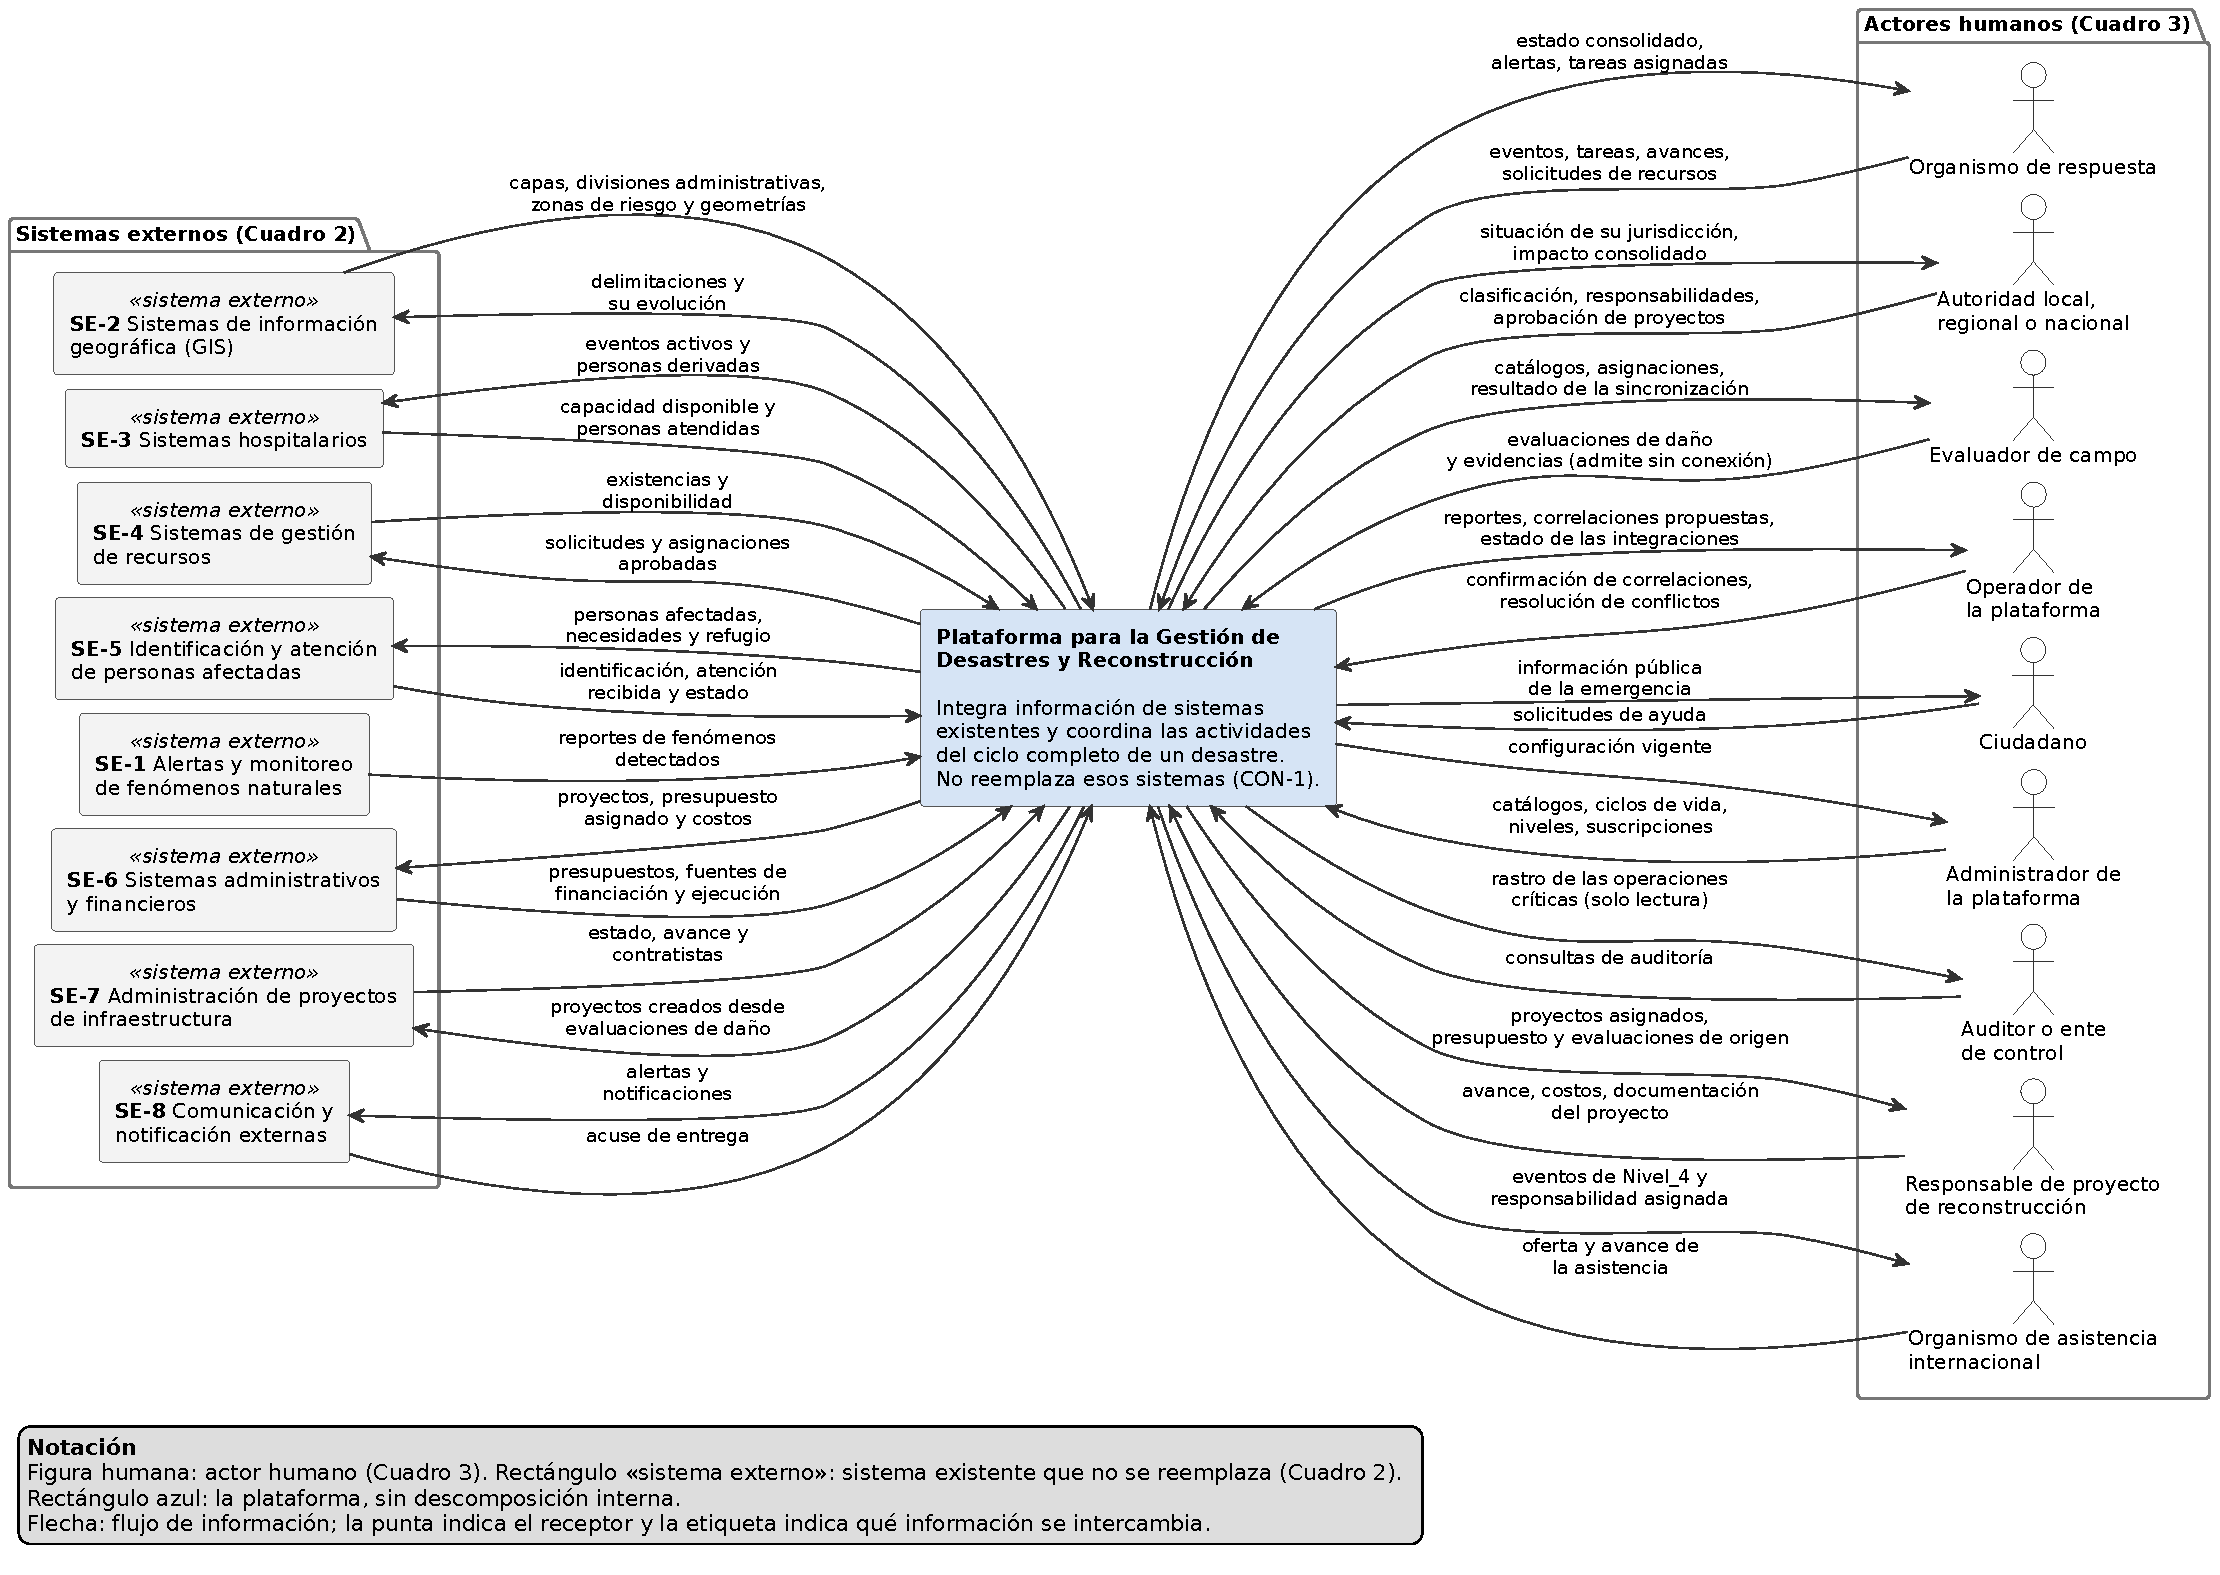
\includegraphics[width=\linewidth,height=0.86\textheight,keepaspectratio]{contexto}
\caption{Diagrama de contexto de la Plataforma para la Gestión de Desastres y Reconstrucción. Cada
flecha indica el sentido del flujo de información según el \cref{tab:externos} y el
\cref{tab:actores}.}
\label{fig:contexto}
\end{figure}
\end{landscape}

%==============================================================================
\newpage
\section{Requisitos funcionales}
\label{sec:requisitos}

\subsection{Convenciones}
\label{sec:convenciones}

Cada requisito se identifica con la forma \texttt{RF-XX-nn}, donde \texttt{XX} es el módulo
(\cref{tab:prefijos}). Los identificadores son estables: no se reutilizan ni se renumeran, y son los
mismos que usan las matrices de la \cref{sec:trazabilidad} y el SAD.

\begin{table}[H]
\centering
\caption{Prefijos de los requisitos funcionales}\label{tab:prefijos}
\begin{tabular}{ll}
\toprule
\textbf{Prefijo} & \textbf{Módulo} \\
\midrule
\texttt{RF-GD} & Gestión de desastres (Módulo 1) \\
\texttt{RF-ED} & Evaluación de daños (Módulo 2) \\
\texttt{RF-PA} & Gestión de personas afectadas (Módulo 3) \\
\texttt{RF-RE} & Gestión de recursos (Módulo 4) \\
\texttt{RF-CO} & Coordinación de organismos (Módulo 5) \\
\texttt{RF-RC} & Reconstrucción (Módulo 6) \\
\bottomrule
\end{tabular}
\end{table}

Los requisitos marcados con \derivado{} son derivados. El equipo de arquitectura los propone a
partir de una exigencia del enunciado, y su descripción indica de cuál se derivan.

La columna de actor usa los nombres del \cref{tab:actores}. \enquote{Autoridad} designa a la
autoridad local, regional o nacional según la jurisdicción del evento. \enquote{Organismo
responsable} designa al organismo de respuesta asignado como responsable del evento.
\enquote{Sin actor iniciador} indica que la plataforma aplica el requisito de forma automática
cuando ocurre la operación a la que se refiere.

La prioridad se asigna con los criterios siguientes:

\begin{description}[leftmargin=1.6cm,labelwidth=1.3cm,labelsep=0.3cm]
  \item[Alta] El requisito realiza una funcionalidad primaria (\cref{tab:primaria}) o un escenario
        calificado (A, A) en el árbol de utilidad: QA-02, QA-03, QA-09 o QA-14
        (\cref{tab:utilidad}).
  \item[Media] El requisito es necesario para completar un módulo, pero no cumple la condición
        anterior. Admite una versión posterior.
  \item[Baja] El requisito mejora la presentación o la consulta de información que otro requisito
        ya ofrece.
\end{description}

Este criterio deja en Alta solo lo que sostiene un objetivo de negocio o uno de los cuatro escenarios
de mayor riesgo: 23 de los 65 requisitos, es decir, el \qty{35}{\percent}.

Cada descripción es comprobable: un tercero puede determinar, mediante la observación del sistema,
si el requisito se cumple, como pide ISO/IEC/IEEE 29148 \cite{iso29148}.

\subsection{Funcionalidad primaria en el sentido de ADD}
\label{sec:primaria}

ADD 3.0 usa como \emph{driver} la funcionalidad primaria, que es la funcionalidad necesaria para
alcanzar los objetivos de negocio que motivan el sistema \cite{cervantes}. El equipo selecciona como
primarios los casos de uso que cumplen dos condiciones: realizan un objetivo del enunciado y
determinan una estructura de la arquitectura. Los demás requisitos se resuelven con las estructuras
que esos casos de uso originan.

El \cref{tab:primaria} identifica diez casos de uso primarios con la forma \texttt{FP-nn}. La versión
1.1 agrega FP-09 y FP-10. Con ellos, los seis módulos tienen al menos un caso de uso primario. En
la versión 1.0, los módulos de personas afectadas y de coordinación de organismos no tenían
ninguno, aunque la coordinación entre organismos y la protección de la información de las personas
afectadas son objetivos explícitos del enunciado.

\begin{longtable}{L{1.5cm} L{5.2cm} L{2.6cm} L{6.1cm}}
\cabecera{4}{tab:primaria}{Funcionalidad primaria y su correspondencia con los requisitos
funcionales}{\textbf{ID} & \textbf{Caso de uso primario} & \textbf{Requisitos} & \textbf{Estructura que determina}}
FP-01 & Registrar un desastre automáticamente a partir de un sistema externo & RF-GD-01 &
El canal de entrada y la traducción de datos externos a un formato interno \\
FP-02 & Consultar y monitorear el estado de un desastre & RF-GD-16 & Un camino de lectura separado
del de escritura, porque este caso de uso recibe la mayor carga concurrente \\
FP-03 & Actualizar la clasificación de severidad y la delimitación geográfica & RF-GD-06, RF-GD-09 &
La conservación de la evolución temporal del evento, además de su valor vigente \\
FP-04 & Consolidar varios reportes de distintas fuentes sobre un mismo evento & RF-GD-11 & Un
mecanismo de correlación y eliminación de duplicados, y el registro de la procedencia de cada dato \\
FP-05 & Notificar a los organismos ante un evento nuevo o un cambio de severidad & RF-GD-15 & Un
canal de salida asíncrono con reintentos y estado de entrega \\
FP-06 & Registrar una evaluación de daños en campo y sincronizarla después & RF-ED-01, RF-ED-12,
RF-ED-13 & Una réplica local en el cliente, la sincronización diferida y una regla determinista de
detección de conflictos \\
FP-07 & Solicitar y asignar un recurso entre organismos & RF-RE-03, RF-RE-04 & Una vista consolidada
de recursos que administran otros sistemas y un mecanismo de reserva que impide asignar dos veces el
mismo recurso \\
FP-08 & Crear un proyecto de reconstrucción a partir de una evaluación de daños & RF-RC-01 & Un
vínculo persistente entre la fase de respuesta y la de reconstrucción, y un registro de cambios
apto para auditoría \\
FP-09 & Asignar responsabilidades y dar seguimiento a las tareas entre organismos & RF-CO-01,
RF-CO-02, RF-CO-05 & La regla de autorización por organismo responsable (QA-11) y el historial de
actividades compartido entre organismos \\
FP-10 & Registrar personas afectadas con protección de sus datos personales & RF-PA-01, RF-PA-08 &
El almacenamiento separado y cifrado de los datos identificatorios y el control de acceso por
necesidad de conocer (QA-12) \\
\end{longtable}

En los cuadros de requisitos, los que forman parte de la funcionalidad primaria llevan la marca (P)
junto a su identificador.

\subsection{Módulo 1: Gestión de desastres}
\label{sec:rf-gd}

Este módulo es el centro de la plataforma. Las evaluaciones de daños, las personas afectadas, las
asignaciones de recursos y los proyectos de reconstrucción se asocian a uno o más eventos de
desastre.

\begin{longtable}{L{2.0cm} L{2.9cm} L{6.0cm} L{3.0cm} L{1.2cm}}
\cabecera{5}{tab:rfgd}{Requisitos funcionales del módulo de Gestión de desastres}{\textbf{ID} &
\textbf{Nombre} & \textbf{Descripción} & \textbf{Actor} & \textbf{Prio.}}
RF-GD-01\prim & Registro automático de evento & El sistema deberá registrar un evento de desastre a
partir de un mensaje recibido de un sistema externo de alerta o monitoreo (SE-1), y conservar la
fuente del mensaje y su marca de tiempo de recepción & SE-1 & AltaAlta \\
RF-GD-02 & Registro manual de evento & El sistema deberá permitir que un usuario autorizado registre
un evento de desastre con los atributos mínimos del \cref{tab:campos-desastre}. El registro podrá
hacerse desde la consola o en campo desde el cliente móvil. En campo, el registro deberá admitirse
sin conexión, con un identificador generado en el cliente, de modo que su reenvío no duplique el
evento (E-42) & Organismo de respuesta (en campo o en la consola), autoridad & Alta \\
RF-GD-03 & Información mínima del evento & El sistema deberá almacenar, para cada evento registrado,
los doce atributos del \cref{tab:campos-desastre}, y rechazar el registro si falta alguno de los
obligatorios & Sin actor iniciador (aplica a RF-GD-01 y RF-GD-02) & Alta \\
RF-GD-04 & Validación contra el catálogo de tipos & El sistema deberá validar el tipo de un evento
contra el catálogo configurable de tipos de desastre (RN-1) y rechazar los tipos no definidos &
Sin actor iniciador (aplica a RF-GD-01 y RF-GD-02) & Alta \\
RF-GD-05 & Clasificación por nivel & El sistema deberá permitir asignar a cada evento uno de los
cuatro niveles de clasificación definidos en RN-3 & Autoridad & Media \\
RF-GD-06\prim & Reclasificación de nivel & El sistema deberá permitir modificar el nivel de un evento
en cualquier momento de su ciclo de vida. Cada reclasificación deberá producir una actualización del
estado del evento, una notificación a los organismos suscritos y una entrada de auditoría con el
valor anterior, el valor nuevo, el autor y la justificación & Autoridad & Alta \\
RF-GD-07 & Transición de estado & El sistema deberá permitir avanzar un evento por su ciclo de vida,
aceptar solo las transiciones válidas para su tipo según la máquina de estados configurable de RN-2
y rechazar las demás & Organismo responsable, autoridad & Media \\
RF-GD-08 & Delimitación geográfica & El sistema deberá permitir definir el área asociada a un evento
a partir de coordenadas, puntos, polígonos, municipios, barrios, zonas de riesgo o geometrías
provistas por un sistema GIS (SE-2), o de una combinación de ellos & Organismo responsable,
autoridad, SE-2 & Media \\
RF-GD-09\prim & Versionado de la delimitación & El sistema deberá conservar cada versión de la
delimitación con su marca de tiempo y su autor, de modo que sea posible reconstruir el área afectada
tal como estaba definida en cualquier instante pasado del evento & Sin actor iniciador (aplica a
RF-GD-08) & Alta \\
RF-GD-10 & Gestión de fuentes de información & El sistema deberá administrar el registro de las
fuentes de información internas y externas de las que puede recibir reportes, con su identificación
y su nivel de confianza & Administrador de la plataforma & Media \\
RF-GD-11\prim & Consolidación de reportes & El sistema deberá consolidar en un único evento los
reportes que distintas fuentes emitan sobre un mismo fenómeno, conservar la procedencia de cada dato
consolidado y escalar a un operador los casos en que la correlación no alcance el nivel de confianza
configurado (RN-6) & Operador de la plataforma & Alta \\
RF-GD-12 & Asociación de organismos & El sistema deberá permitir asociar a un evento los organismos
participantes, e indicar la responsabilidad de cada uno y cuál de ellos es el responsable asignado
del evento. El sistema deberá proponer los organismos que el tipo y el nivel del evento definen por
defecto (RN-1) & Autoridad & Media \\
RF-GD-13 & Visualización de participantes & El sistema deberá presentar, para un evento dado, los
organismos que participan y la responsabilidad de cada uno & Todos los actores autorizados & Baja \\
RF-GD-14 & Priorización de tareas del evento & El sistema deberá permitir asignar y modificar la
prioridad de las tareas asociadas a un evento & Organismo responsable, autoridad & Media \\
RF-GD-15\prim & Generación de alertas y notificaciones & El sistema deberá generar una notificación
dirigida a los organismos suscritos cuando se cree un evento o cambie su nivel, y deberá registrar
para cada notificación su estado de entrega (pendiente, entregada o fallida) & Sin actor iniciador.
Destinatarios: organismos suscritos, por medio de SE-8 & Alta \\
RF-GD-16\prim & Consulta y monitoreo del evento & El sistema deberá presentar el estado consolidado
de un evento (nivel, estado del ciclo de vida, delimitación vigente, organismos participantes y
resumen de daños) con la marca de tiempo del dato mostrado & Todos los actores autorizados & Alta \\
RF-GD-17 & Consulta de la evolución del evento & El sistema deberá presentar la evolución de un
evento en el tiempo: cambios de nivel, cambios de estado y cambios de delimitación, en orden
cronológico & Autoridad, auditor & Baja \\
RF-GD-18 & Cierre del evento & El sistema deberá permitir cerrar un evento cuando su tipo admita la
transición al estado Cerrado, y registrar el autor, la fecha y la justificación del cierre &
Autoridad & Media \\
\end{longtable}

El \cref{tab:campos-desastre} define la información mínima de registro de un desastre. La versión
1.1 precisa el origen de la ubicación geográfica y la multiplicidad de los atributos 6, 9 y 12.

\begin{longtable}{L{0.7cm} L{3.2cm} L{7.5cm} L{2.6cm} L{1.2cm}}
\cabecera{5}{tab:campos-desastre}{Información mínima de registro de un evento de desastre (doce
atributos)}{\textbf{N.º} & \textbf{Atributo} & \textbf{Descripción y reglas} & \textbf{Multiplicidad} & \textbf{Oblig.}}
1 & Identificador único & Identificador único en todo el sistema e inmutable. En un registro en
campo lo genera el cliente móvil de forma que no colisione aunque se genere sin conexión (RF-GD-02,
E-42) & 1 & Sí \\
2 & Tipo de desastre & Referencia a una entrada vigente del catálogo de tipos (RN-1) & 1 & Sí \\
3 & Fecha y hora de inicio & Instante estimado de inicio del fenómeno, con zona horaria explícita &
1 & Sí \\
4 & Ubicación geográfica & Coordenadas del punto de referencia del evento. Su origen es el punto
que informa la fuente del reporte: en un registro automático, la ubicación que reporta SE-1 (por
ejemplo, el epicentro de un sismo); en un registro manual, el punto que indica el usuario. El
origen queda registrado en el atributo 8 & 1 & Sí \\
5 & Área o zonas potencialmente afectadas & Delimitación vigente del evento (RN-4). Cada cambio
conserva la versión anterior & 1 vigente, N históricas & Sí \\
6 & Nivel de severidad & Uno de los cuatro niveles de RN-3. Cada reclasificación conserva el nivel
anterior (RF-GD-06) & 1 vigente, N históricos & Sí \\
7 & Descripción del evento & Texto libre que describe el fenómeno y su situación & 1 & Sí \\
8 & Fuente de la información & Fuente de la que proviene cada reporte: SE-1, otro sistema externo o
un usuario. Se conserva por cada dato consolidado (RN-6) & 1..N & Sí \\
9 & Organismo que registra el evento & Organización que efectuó el registro. Cuando varios
organismos reportan el mismo fenómeno, se conservan todos (RN-6). Puede ser distinto del responsable
de la emergencia & 1..N & Sí \\
10 & Responsable de la emergencia & Organismo responsable asignado. Determina quién puede modificar
el evento (QA-11). Sus datos de contacto son información sensible & 1 & Sí \\
11 & Estado actual & Estado vigente dentro del ciclo de vida configurado para el tipo (RN-2) & 1 &
Sí \\
12 & Fecha y hora de actualización & Instante de cada modificación del evento, con zona horaria
explícita. El valor vigente es el de la última modificación & 1 vigente, N históricas & Sí \\
\end{longtable}

Además de los doce atributos, el evento tiene un nombre: una etiqueta corta de presentación, como
\enquote{Sismo de Pasto}, que identifica el evento en listas y mapas (E-30). El nombre no forma
parte de la información mínima del enunciado y no reemplaza al atributo 7. La implementación lo
exige en el registro, porque las copias locales de otros módulos lo muestran (SAD 1.2, EV-03)
\cite{sad}.

\subsection{Módulo 2: Evaluación de daños}
\label{sec:rf-ed}

\begin{longtable}{L{2.0cm} L{2.9cm} L{6.0cm} L{3.0cm} L{1.2cm}}
\cabecera{5}{tab:rfed}{Requisitos funcionales del módulo de Evaluación de daños}{\textbf{ID} &
\textbf{Nombre} & \textbf{Descripción} & \textbf{Actor} & \textbf{Prio.}}
RF-ED-01\prim & Registro de evaluación & El sistema deberá permitir registrar una evaluación de
daños sobre un activo afectado con los once atributos del \cref{tab:campos-evaluacion}. El sistema
deberá asignar a cada activo la división administrativa que contiene su ubicación (E-12) & Evaluador
de campo & Alta \\
RF-ED-02 & Información mínima de la evaluación & El sistema deberá almacenar, para cada evaluación,
los once atributos del \cref{tab:campos-evaluacion}, y rechazar el registro si falta alguno de los
obligatorios & Sin actor iniciador (aplica a RF-ED-01) & Alta \\
RF-ED-03 & Adjuntar evidencias & El sistema deberá permitir adjuntar a una evaluación fotografías,
documentos y coordenadas geográficas como evidencia, y conservar para cada evidencia su autor y su
marca de tiempo de captura & Evaluador de campo & Alta \\
RF-ED-04 & Catálogo de tipos de activo & El sistema deberá administrar un catálogo configurable de
tipos de activo evaluables (vivienda, edificio público, hospital, escuela, puente, carretera,
sistema de agua, red eléctrica, red de telecomunicaciones, instalación industrial y otra
infraestructura crítica). La ampliación del catálogo no deberá requerir la modificación de
componentes & Administrador de la plataforma & Media \\
RF-ED-05 & Categorías de daño configurables & El sistema deberá permitir que el administrador
configure, por tipo de activo, los criterios que llevan a cada categoría de daño (RN-5), y que el
evaluador clasifique el daño de un activo con esas categorías & Administrador de la plataforma
(configura); evaluador de campo (clasifica) & Media \\
RF-ED-06 & Asociación al desastre y registro preliminar & El sistema deberá asociar cada evaluación
a un desastre registrado. Deberá admitir el registro de evaluaciones preliminares no asociadas
cuando aún no exista información suficiente para identificar el evento, y permitir su asociación
posterior & Evaluador de campo, operador de la plataforma & Media \\
RF-ED-07 & Actualización de una evaluación & El sistema deberá permitir actualizar una evaluación
existente y conservar la versión anterior con su marca de tiempo y su autor & Evaluador de campo &
Alta \\
RF-ED-08 & Validación de evaluaciones & El sistema deberá permitir que un usuario autorizado marque
una evaluación como validada, rechazada o pendiente, y registrar quién lo hizo y cuándo & Organismo
responsable, autoridad & Media \\
RF-ED-09 & Gestión de duplicidad & El sistema deberá detectar las evaluaciones que se refieran al
mismo activo dentro de una ventana de tiempo configurable, marcarlas como posibles duplicados y
permitir que un usuario autorizado las fusione o las rechace. Fusionar dos evaluaciones marcadas
como posible duplicado significa elegir una como vigente y marcar la otra como duplicada de ella.
La evaluación duplicada conserva todas sus versiones y sus evidencias. Sus evidencias quedan
vinculadas también a la evaluación vigente. Ninguna versión ni evidencia se elimina (E-14) &
Operador de la plataforma & Media \\
RF-ED-10 & Priorización y estimación de impacto & El sistema deberá calcular, a partir de las
evaluaciones validadas de un desastre, un consolidado del impacto por zona y por tipo de activo que
permita establecer prioridades de atención & Autoridad & Media \\
RF-ED-11 & Visualización geográfica de daños & El sistema deberá presentar sobre un mapa las zonas
afectadas y su nivel de daño consolidado & Autoridad, organismo de respuesta & Media \\
RF-ED-12\prim & Operación sin conexión & El sistema deberá permitir que un evaluador descargue
previamente la información necesaria, registre evaluaciones y capture evidencias sin conectividad,
y almacene esos registros localmente hasta recuperar la conexión & Evaluador de campo & Alta \\
RF-ED-13\prim & Sincronización y conflictos & El sistema deberá sincronizar las evaluaciones
registradas sin conexión cuando se recupere la conectividad. Deberá detectar los conflictos con
modificaciones ocurridas entretanto mediante una regla determinista que no dependa de los relojes de
los dispositivos (S-5), conservar ambas versiones y escalar la resolución a un usuario autorizado.
No deberá descartar información de forma automática & Evaluador de campo, operador de la plataforma
& Alta \\
RF-ED-14 & Publicación de eventos hacia otros módulos & El sistema deberá publicar el resultado de
una evaluación validada de modo que los módulos de recursos y de reconstrucción puedan consumirlo
sin consultar directamente el almacén de evaluaciones & Sin actor iniciador (aplica a RF-ED-08) &
Media \\
RF-ED-15 & Seguimiento de la evolución de los daños & El sistema deberá presentar, para un activo o
una zona, la secuencia de evaluaciones registradas en el tiempo con su nivel de daño & Autoridad &
Baja \\
\end{longtable}

El \cref{tab:campos-evaluacion} define la información mínima de registro de una evaluación de daños.

\begin{longtable}{L{0.7cm} L{3.2cm} L{7.5cm} L{2.6cm} L{1.2cm}}
\cabecera{5}{tab:campos-evaluacion}{Información mínima de registro de una evaluación de daños (once
atributos)}{\textbf{N.º} & \textbf{Atributo} & \textbf{Descripción y reglas} & \textbf{Multiplicidad} & \textbf{Oblig.}}
1 & Identificador & Identificador único de la evaluación, asignado de forma que no colisione aunque
se genere sin conexión (RF-ED-12) & 1 & Sí \\
2 & Desastre asociado & Referencia al evento de desastre. Puede quedar vacío en una evaluación
preliminar y asociarse después (RF-ED-06) & 0..1 & No\,(*) \\
3 & Fecha y hora & Instante de la evaluación en campo según el dispositivo. El instante de recepción
en el servidor se conserva por separado, junto con el desfase del reloj del dispositivo (S-5) & 1 &
Sí \\
4 & Evaluador & Persona que realizó la evaluación & 1 & Sí \\
5 & Organización & Organización a la que pertenece el evaluador & 1 & Sí \\
6 & Ubicación geográfica & Coordenadas del activo evaluado & 1 & Sí \\
6\derivado & Municipio del activo (\texttt{codigo\-Municipio}) & Atributo derivado. Lo calcula el
servidor a partir de la ubicación (atributo 6) y no se pide al evaluador (E-12) & 1 & No\newline (**) \\
7 & Tipo de activo afectado & Referencia a una entrada del catálogo de tipos de activo (RF-ED-04) &
1 & Sí \\
8 & Nivel de daño & Categoría de daño aplicable al tipo de activo, según RN-5 & 1 & Sí \\
9 & Descripción & Texto libre que describe el daño observado & 1 & Sí \\
10 & Evidencias & Fotografías, documentos y coordenadas adjuntas & 0..N & No \\
11 & Estado de la evaluación & Estado de la evaluación en la plataforma: preliminar, registrada, en
conflicto, validada o rechazada. El estado local de sincronización (pendiente, confirmada o
inválida) es un dato distinto. Pertenece a la réplica local del dispositivo e indica si el servidor
ya respondió a la operación. No forma parte de este atributo & 1 & Sí \\
\end{longtable}

(*) El atributo \enquote{Desastre asociado} es obligatorio, con una excepción: la evaluación
preliminar que admite RF-ED-06.

(**) El municipio del activo no cuenta entre los once atributos de registro, porque el evaluador no
lo ingresa. El servidor lo asigna en toda evaluación aceptada, y la consulta por zona lo usa
(RF-ED-10, RF-ED-11).

\subsection{Módulo 3: Gestión de personas afectadas}
\label{sec:rf-pa}

\begin{longtable}{L{2.0cm} L{2.9cm} L{6.0cm} L{3.0cm} L{1.2cm}}
\cabecera{5}{tab:rfpa}{Requisitos funcionales del módulo de Gestión de personas
afectadas}{\textbf{ID} & \textbf{Nombre} & \textbf{Descripción} & \textbf{Actor} & \textbf{Prio.}}
RF-PA-01\prim & Registro de personas afectadas & El sistema deberá registrar las personas afectadas
por un desastre e integrar la información que aporten los sistemas de identificación y atención
(SE-5), sin reemplazarlos & Organismo de respuesta, SE-5 & Alta \\
RF-PA-02 & Registro de familias & El sistema deberá permitir agrupar personas afectadas en familias
y mantener el vínculo entre ellas & Organismo de respuesta & Media \\
RF-PA-03 & Registro de necesidades & El sistema deberá registrar las necesidades declaradas o
identificadas de una persona o familia afectada & Organismo de respuesta & Media \\
RF-PA-04 & Ubicación de la persona afectada & El sistema deberá registrar la ubicación actual de una
persona o familia afectada y su historial de ubicaciones & Organismo de respuesta & Media \\
RF-PA-05 & Gestión de refugios & El sistema deberá registrar los refugios habilitados, su capacidad
y su ocupación actual, y permitir asociar personas afectadas a un refugio & Organismo de respuesta,
autoridad & Media \\
RF-PA-06 & Registro de atención recibida & El sistema deberá registrar la atención recibida por una
persona afectada, con el organismo que la prestó y la fecha & Organismo de respuesta & Media \\
RF-PA-07 & Solicitudes de ayuda & El sistema deberá registrar solicitudes de ayuda, asociarlas a
una persona o familia y permitir el seguimiento de su estado hasta su cierre & Ciudadano, organismo
de respuesta & Media \\
RF-PA-08\prim & Protección de datos personales & El sistema deberá restringir el acceso a los datos
identificatorios de las personas afectadas a los roles con necesidad de conocer, y deberá presentar
información agregada o seudonimizada a los demás & Sin actor iniciador (aplica a toda consulta del
módulo) & Alta \\
RF-PA-09 & Trazabilidad de cambios & El sistema deberá registrar toda creación, modificación,
consulta y eliminación de información de personas afectadas, con quién la hizo, qué hizo, cuándo,
sobre qué información y con qué resultado & Sin actor iniciador. Destinatario: auditor & Media \\
\end{longtable}

\subsection{Módulo 4: Gestión de recursos}
\label{sec:rf-re}

\begin{longtable}{L{2.0cm} L{2.9cm} L{6.0cm} L{3.0cm} L{1.2cm}}
\cabecera{5}{tab:rfre}{Requisitos funcionales del módulo de Gestión de recursos}{\textbf{ID} &
\textbf{Nombre} & \textbf{Descripción} & \textbf{Actor} & \textbf{Prio.}}
RF-RE-01 & Registro de recursos & El sistema deberá registrar recursos de las categorías siguientes:
alimentos, agua, medicamentos, vehículos, maquinaria, equipos de rescate, personal, refugios y
donaciones. Para cada recurso deberá registrar su cantidad, su ubicación y la organización que lo
posee & Organismo de respuesta, administrador de la plataforma & Media \\
RF-RE-02 & Visión consolidada de disponibilidad & El sistema deberá presentar una visión
consolidada de los recursos disponibles que integre la información de los sistemas de gestión de
recursos (SE-4), con la fuente y la marca de tiempo de cada dato & Autoridad, organismo de respuesta
& Media \\
RF-RE-03\prim & Solicitud de recursos & El sistema deberá permitir que un organismo autorizado
solicite recursos con la cantidad, el destino y el desastre asociado, y deberá mantener el estado de
la solicitud hasta su cierre & Organismo de respuesta & Alta \\
RF-RE-04\prim & Asignación de recursos & El sistema deberá permitir asignar recursos a una solicitud
y descontar la cantidad asignada de la disponibilidad presentada, de modo que un mismo recurso no
quede asignado simultáneamente a dos solicitudes & Autoridad, organismo de respuesta autorizado &
Alta \\
RF-RE-05 & Registro de donaciones & El sistema deberá registrar las donaciones recibidas, con el
donante, el contenido, la fecha y el destino asignado & Organismo de respuesta & Media \\
RF-RE-06 & Trazabilidad de la asignación & El sistema deberá registrar cada solicitud y cada
asignación de recursos, con quién la hizo, qué hizo, cuándo, sobre qué recurso y con qué resultado &
Sin actor iniciador. Destinatario: auditor & Media \\
RF-RE-07 & Publicación hacia sistemas externos & El sistema deberá comunicar a los sistemas de
gestión de recursos (SE-4) las asignaciones aprobadas, y deberá conservarlas como pendientes si el
sistema externo no está disponible & Sin actor iniciador. Destinatario: SE-4 & Media \\
\end{longtable}

\subsection{Módulo 5: Coordinación de organismos}
\label{sec:rf-co}

\begin{longtable}{L{2.0cm} L{2.9cm} L{6.0cm} L{3.0cm} L{1.2cm}}
\cabecera{5}{tab:rfco}{Requisitos funcionales del módulo de Coordinación de organismos}{\textbf{ID} &
\textbf{Nombre} & \textbf{Descripción} & \textbf{Actor} & \textbf{Prio.}}
RF-CO-01\prim & Asignar responsabilidades & El sistema deberá permitir asignar a cada organismo
participante una responsabilidad definida dentro de un desastre & Autoridad & Alta \\
RF-CO-02\prim & Crear tareas & El sistema deberá permitir crear tareas asociadas a un desastre, con
el organismo o la persona responsable, la descripción y la fecha límite & Organismo de respuesta,
autoridad & Alta \\
RF-CO-03 & Establecer prioridades & El sistema deberá permitir asignar y modificar la prioridad de
una tarea, y presentar las tareas ordenadas por prioridad & Organismo de respuesta, autoridad &
Media \\
RF-CO-04 & Compartir información & El sistema deberá permitir que un organismo publique información
asociada a un desastre y que los demás organismos participantes la consulten, según las reglas de
acceso vigentes & Organismo de respuesta, organismo de asistencia internacional & Media \\
RF-CO-05\prim & Registrar avances & El sistema deberá permitir registrar el avance de una tarea, con
su autor y su marca de tiempo, hasta su cierre & Organismo de respuesta, organismo de asistencia
internacional & Alta \\
RF-CO-06 & Generar alertas de coordinación & El sistema deberá generar alertas dirigidas a los
organismos participantes ante los eventos de coordinación configurados, como una tarea vencida o una
nueva responsabilidad asignada & Sin actor iniciador. Destinatarios: organismos participantes &
Media \\
RF-CO-07 & Historial de actividades & El sistema deberá mantener y presentar el historial de
actividades de coordinación de un desastre en orden cronológico & Autoridad, auditor & Baja \\
\end{longtable}

\subsection{Módulo 6: Reconstrucción}
\label{sec:rf-rc}

\begin{longtable}{L{2.0cm} L{2.9cm} L{6.0cm} L{3.0cm} L{1.2cm}}
\cabecera{5}{tab:rfrc}{Requisitos funcionales del módulo de Reconstrucción}{\textbf{ID} &
\textbf{Nombre} & \textbf{Descripción} & \textbf{Actor} & \textbf{Prio.}}
RF-RC-01\prim & Crear proyecto desde una evaluación & El sistema deberá permitir crear un proyecto
de recuperación o reconstrucción a partir de una o más evaluaciones de daño validadas, y conservar
el vínculo con las evaluaciones que lo originaron & Autoridad & Alta \\
RF-RC-02 & Información del proyecto & El sistema deberá almacenar, para cada proyecto, presupuesto,
fuente de financiación, responsable, contratista, cronograma, avance, costos, documentación,
evidencias y estado del proyecto & Sin actor iniciador (aplica a RF-RC-01) & Media \\
RF-RC-03 & Asignar presupuesto y responsable & El sistema deberá permitir asignar y modificar el
presupuesto, la fuente de financiación y el responsable de un proyecto & Autoridad & Media \\
RF-RC-04 & Registrar avance & El sistema deberá permitir registrar el avance de un proyecto con su
marca de tiempo y su autor & Responsable de proyecto de reconstrucción & Media \\
RF-RC-05 & Registrar costos & El sistema deberá permitir registrar los costos ejecutados de un
proyecto y compararlos con el presupuesto asignado & Responsable de proyecto de reconstrucción &
Media \\
RF-RC-06 & Documentación y evidencias & El sistema deberá permitir adjuntar documentación y
evidencias a un proyecto, y conservar su autor y su marca de tiempo & Responsable de proyecto de
reconstrucción & Media \\
RF-RC-07 & Auditoría de presupuesto y estado & El sistema deberá registrar todo cambio de
presupuesto y todo cambio de estado de un proyecto, con el valor anterior, el valor nuevo, el autor,
la justificación y la marca de tiempo. El registro no deberá poder modificarse ni eliminarse &
Sin actor iniciador. Destinatario: auditor & Media \\
RF-RC-08\derivado & Creación de proyectos por lote & El sistema deberá permitir crear proyectos para
un conjunto de activos evaluados en una sola operación, y conservar el vínculo de cada proyecto con
su evaluación de origen. Se deriva del escenario EO-5, en el que la autoridad interviene un conjunto
de activos (por ejemplo, 30 escuelas y 12 puentes) & Autoridad & Media \\
RF-RC-09\derivado & Consulta consolidada del programa & El sistema deberá presentar el estado
consolidado del conjunto de proyectos de un desastre: número de proyectos por estado, presupuesto
asignado, costo ejecutado y avance agregado. Se deriva de la exigencia de dar seguimiento al avance
de los proyectos, aplicada al conjunto de proyectos de un desastre & Autoridad, auditor & Baja \\
\end{longtable}

\subsection{Resumen}

\begin{table}[H]
\centering
\caption{Resumen de los requisitos funcionales por módulo}\label{tab:resumen}
\small\setlength{\tabcolsep}{4pt}
\begin{tabular}{lcccccl}
\toprule
\textbf{Módulo} & \textbf{Requisitos} & \textbf{Primarios} & \textbf{Alta} & \textbf{Media} &
\textbf{Baja} & \textbf{Rango de identificadores} \\
\midrule
Gestión de desastres          & 18 & 6 & 9 & 7 & 2 & RF-GD-01 a RF-GD-18 \\
Evaluación de daños           & 15 & 3 & 6 & 8 & 1 & RF-ED-01 a RF-ED-15 \\
Gestión de personas afectadas & 9  & 2 & 2 & 7 & 0 & RF-PA-01 a RF-PA-09 \\
Gestión de recursos           & 7  & 2 & 2 & 5 & 0 & RF-RE-01 a RF-RE-07 \\
Coordinación de organismos    & 7  & 3 & 3 & 3 & 1 & RF-CO-01 a RF-CO-07 \\
Reconstrucción                & 9  & 1 & 1 & 7 & 1 & RF-RC-01 a RF-RC-09 \\
\midrule
Total                         & 65 & 17 & 23 & 37 & 5 & \\
\bottomrule
\end{tabular}
\end{table}

De los 65 requisitos, 63 son exigencias directas del enunciado y 2 son derivados (RF-RC-08 y
RF-RC-09). Los 17 requisitos primarios corresponden a los 10 casos de uso primarios del
\cref{tab:primaria}. La versión 1.2 reclasifica los 65 requisitos con el criterio de la
\cref{sec:convenciones}: 23 en Alta (\qty{35}{\percent}), 37 en Media (\qty{57}{\percent}) y 5 en
Baja (\qty{8}{\percent}). Los 23 de prioridad Alta son los 17 primarios y seis requisitos que realizan
escenarios (A, A): RF-GD-02, RF-GD-03 y RF-GD-04 (el registro de eventos, servicio crítico de QA-02) y
RF-ED-02, RF-ED-03 y RF-ED-07 (la información, las evidencias y las versiones que QA-14 protege).

%==============================================================================
\newpage
\section{Reglas de negocio}
\label{sec:reglas}

El enunciado exige que tres aspectos del dominio sean configurables: los tipos de desastre que
existen, los estados por los que pasa cada tipo y el nivel de gravedad de cada desastre. Los tres
se refieren a los tipos de desastre, pero son ejes de variabilidad independientes, con estructuras
de datos distintas. Un tipo nuevo no implica un estado nuevo. Un cambio de nivel no implica un
cambio de tipo. El ciclo de vida de un terremoto difiere del de una inundación aunque ambos alcancen
el Nivel\_4. Por esta razón el documento los especifica como reglas separadas (RN-1, RN-2 y RN-3).
Las reglas RN-4 a RN-6 especifican la delimitación geográfica, las categorías de daño y la
consolidación de fuentes.

\subsection{RN-1: Catálogo de tipos de desastre}

La plataforma administra un catálogo de tipos de desastre. El catálogo es contenido que se
administra en tiempo de ejecución. Incorporar un tipo, retirarlo o modificar sus atributos no
requiere modificar ni redesplegar ningún componente de la plataforma.

El contenido inicial del catálogo es: terremoto, inundación, incendio, deslizamiento, huracán,
erupción volcánica y otros eventos que defina la organización \cite{enunciado}. El
\cref{tab:catalogo} lista los atributos de una entrada.

\begin{table}[H]
\centering
\caption{Atributos de una entrada del catálogo de tipos de desastre}\label{tab:catalogo}
\begin{tabular}{L{4.2cm} L{11.4cm}}
\toprule
\textbf{Atributo} & \textbf{Descripción} \\
\midrule
Código & Identificador estable del tipo, inmutable una vez creado \\
Nombre & Denominación que se presenta a los usuarios \\
Perfil de ciclo de vida & Referencia al perfil de máquina de estados aplicable (RN-2) \\
Criterios de clasificación & Referencia al conjunto de criterios de nivel aplicables (RN-3) \\
Categorías de daño aplicables & Referencia a los criterios de daño por tipo de activo (RN-5) \\
Organismos convocados por defecto & Organismos de respuesta que se proponen como participantes al
registrar un evento de este tipo, por nivel de clasificación (RF-GD-12) \\
Categorías de recursos requeridas por defecto & Categorías de recursos que se proponen al crear las
solicitudes de un evento de este tipo (RF-RE-03) \\
Vigencia & Período durante el cual el tipo puede usarse para registrar eventos nuevos \\
\bottomrule
\end{tabular}
\end{table}

El tipo de un evento, junto con su nivel (RN-3), determina los organismos que participan y los
recursos que se requieren por defecto. La autoridad puede ajustar ambos conjuntos en cada evento.
Los dos atributos correspondientes se agregan en la versión 1.1.

Un tipo retirado deja de estar disponible para registrar eventos nuevos, pero permanece en el
catálogo. Los eventos históricos registrados con ese tipo conservan su referencia y siguen siendo
consultables. El catálogo cambia la vigencia de una entrada y no la elimina.

Esta regla tiene una consecuencia sobre el diseño. La lógica del módulo de gestión de desastres
opera sobre un evento genérico y consulta el catálogo en ejecución, sin conocer los tipos concretos.
Esta regla sustenta el escenario QA-10.

\subsection{RN-2: Ciclo de vida y máquina de estados configurable}

Todo evento de desastre tiene un estado dentro de un ciclo de vida. Los estados posibles son siete:
Detectado, Registrado, En evaluación, En atención, En recuperación, En reconstrucción y Cerrado.
Las transiciones válidas dependen del tipo de desastre. Cada tipo tiene asociado un perfil de ciclo
de vida, que define las transiciones que se admiten. Un evento de baja gravedad puede pasar de
Registrado a Cerrado. Un terremoto de gran magnitud puede permanecer semanas o meses en las fases
intermedias \cite{enunciado}.

El \cref{tab:transiciones} define el conjunto máximo de transiciones admisibles. Un perfil de ciclo
de vida es un subconjunto de este cuadro. Ningún perfil puede definir una transición que no
aparezca en él.

\begin{longtable}{L{3.0cm} L{4.4cm} L{8.4cm}}
\cabecera{3}{tab:transiciones}{Transiciones válidas del ciclo de vida de un evento de
desastre}{\textbf{Estado origen} & \textbf{Estado destino admisible} & \textbf{Condición y observaciones}}
(inicial) & Detectado & Creación automática a partir de un reporte de SE-1 (RF-GD-01) \\
(inicial) & Registrado & Creación manual por un usuario autorizado (RF-GD-02) \\
Detectado & Registrado & Un usuario autorizado confirma el evento y completa la información mínima \\
Detectado & Cerrado & El reporte se descarta por falsa alarma. Requiere una justificación
registrada \\
Registrado & En evaluación & Se despliegan equipos de campo o se solicita una evaluación de daños \\
Registrado & En atención & El evento requiere respuesta inmediata sin evaluación previa \\
Registrado & Cerrado & Ruta corta para un evento de baja gravedad que no requiere fases
intermedias \\
En evaluación & En atención & Se inicia la respuesta operativa \\
En evaluación & En recuperación & La evaluación concluye que no hay respuesta de emergencia
pendiente \\
En evaluación & Cerrado & La evaluación concluye que no hay impacto que atender \\
En atención & En evaluación & La autoridad ordena una nueva evaluación de daños por un cambio en la
situación \\
En atención & En recuperación & Concluye la fase de respuesta de emergencia \\
En atención & Cerrado & El evento se resuelve sin fase de recuperación \\
En recuperación & En reconstrucción & Se crean proyectos de reconstrucción (RF-RC-01) \\
En recuperación & Cerrado & No se requieren proyectos de reconstrucción \\
En reconstrucción & Cerrado & Todos los proyectos asociados alcanzan un estado final \\
Cerrado & En atención & Reapertura. Solo la autoridad nacional puede ordenarla, con justificación
obligatoria y entrada de auditoría. No forma parte de ningún perfil estándar \\
\end{longtable}

Toda transición a Cerrado exige una condición adicional, cualquiera que sea el estado de origen:
todos los proyectos de reconstrucción asociados al evento deben estar finalizados o cancelados
(E-07). Si un proyecto asociado está en otro estado, la plataforma rechaza la transición e informa
cuántos proyectos siguen abiertos (RF-GD-07, RF-GD-18). Gestión de desastres conoce el estado de
los proyectos por los eventos que publica Reconstrucción (SAD 1.2, AD-47) \cite{sad}.

El \cref{tab:perfiles} propone tres perfiles iniciales. La organización puede definir otros.

\begin{table}[H]
\centering
\caption{Perfiles de ciclo de vida propuestos}\label{tab:perfiles}
\begin{tabular}{L{2.6cm} L{6.4cm} L{6.6cm}}
\toprule
\textbf{Perfil} & \textbf{Estados que recorre} & \textbf{Aplicación habitual} \\
\midrule
Simplificado & Registrado, Cerrado & Eventos de Nivel\_1 atendidos con recursos locales. Perfil
mínimo del Nivel\_1 \\
Estándar & Detectado, Registrado, En evaluación, En atención, En recuperación, Cerrado &
Incendios, deslizamientos e inundaciones de alcance municipal. Perfil mínimo del Nivel\_2 \\
Extendido & Los siete estados, incluido En reconstrucción & Terremotos, huracanes y erupciones
volcánicas con daño estructural. Perfil mínimo del Nivel\_3 y del Nivel\_4 \\
\bottomrule
\end{tabular}
\end{table}

Cada nivel de RN-3 tiene un perfil mínimo (E-35): Simplificado para el Nivel\_1, Estándar para el
Nivel\_2 y Extendido para el Nivel\_3 y el Nivel\_4. La asignación de perfil mínimo por nivel es
configurable en ejecución por el administrador de la plataforma (QA-10). Al registrarse, un evento
recibe el perfil de su tipo, salvo que el perfil mínimo de su nivel sea superior. En ese caso
recibe el perfil mínimo del nivel.

Si un evento se reclasifica a un nivel superior (RN-3) y su perfil es inferior al perfil mínimo del
nuevo nivel, el evento cambia a ese perfil mínimo. El cambio de perfil conserva los estados ya
recorridos. Una reclasificación a un nivel inferior no reduce el perfil.

Esta regla exige una máquina de estados dirigida por datos. El componente que valida una transición
consulta en ejecución el perfil aplicable y no tiene las transiciones escritas en su lógica. Esta
regla también sustenta QA-10.

\subsection{RN-3: Niveles de clasificación}

Todo evento de desastre tiene asignado un nivel, que expresa su impacto y la atención que requiere.
El \cref{tab:niveles} define los cuatro niveles \cite{enunciado}.

\begin{table}[H]
\centering
\caption{Niveles de clasificación de un evento de desastre}\label{tab:niveles}
\begin{tabular}{L{3.0cm} L{7.4cm} L{5.2cm}}
\toprule
\textbf{Nivel} & \textbf{Definición} & \textbf{Ámbito de coordinación} \\
\midrule
Nivel\_1 (Bajo) & Puede atenderse con recursos locales & Autoridad local \\
Nivel\_2 (Medio) & Requiere coordinación entre varios organismos & Autoridad local y varios
organismos \\
Nivel\_3 (Alto) & Requiere recursos regionales o nacionales & Autoridad regional o nacional \\
Nivel\_4 (Crítico) & Requiere coordinación nacional y posiblemente asistencia internacional &
Autoridad nacional y, si esta lo decide, organismos de asistencia internacional \\
\bottomrule
\end{tabular}
\end{table}

La clasificación puede modificarse en cualquier momento, a medida que se dispone de información
nueva. Por ejemplo, un evento clasificado como Nivel\_1 puede pasar a Nivel\_3. La reclasificación
es parte del comportamiento esperado de una emergencia.

Toda reclasificación, ascendente o descendente, produce tres efectos:

\begin{enumerate}
  \item La actualización del estado de la emergencia, incluido el cambio al perfil mínimo del nuevo
        nivel cuando el perfil vigente es inferior (RN-2, \cref{tab:perfiles}, E-35).
  \item La notificación a los organismos suscritos al nuevo ámbito de coordinación del
        \cref{tab:niveles}. Un ascenso de Nivel\_1 a Nivel\_3 incorpora destinatarios nuevos.
  \item El registro para trazabilidad: una entrada de auditoría con el nivel anterior, el nivel
        nuevo, el autor, la marca de tiempo y la justificación.
\end{enumerate}

El usuario percibe los tres efectos como una sola operación. Si la notificación no puede entregarse,
el cambio queda registrado y la notificación permanece en estado pendiente, con reintento. Una
notificación solo pasa al estado entregada cuando existe acuse de entrega.

Los criterios para asignar un nivel son configurables por tipo de desastre. Los criterios de un
terremoto (magnitud, población en el área, daño estructural reportado) difieren de los de una
inundación (área inundada, viviendas afectadas, personas evacuadas). La plataforma administra los
criterios y la organización los define (S-3).

En esta regla coinciden tres atributos de calidad: la modificabilidad, porque los criterios son
configurables (QA-10); la trazabilidad (QA-13); y el rendimiento, porque la notificación resultante
debe cumplir QA-08.

\subsection{RN-4: Delimitación geográfica versionada}

El área asociada a un desastre se define a partir de coordenadas, puntos geográficos, polígonos,
municipios, barrios, zonas de riesgo o información de sistemas GIS (SE-2), o de una combinación de
estas fuentes.

La delimitación cambia en el tiempo. Por ejemplo, a las 10:00 se estima que el área afectada
comprende 3 barrios y a las 14:00 una evaluación determina que se extendió a 7 barrios
\cite{enunciado}.

Cada versión de la delimitación se conserva con su marca de tiempo, su autor y su fuente
(\cref{tab:delimitacion}). Una delimitación nueva sucede a la anterior y no la sobrescribe. La
plataforma debe poder informar el área afectada en cualquier instante pasado y reconstruir la
evolución espacial del evento.

\begin{table}[H]
\centering
\caption{Atributos de una versión de la delimitación geográfica}\label{tab:delimitacion}
\begin{tabular}{L{2.6cm} L{13.0cm}}
\toprule
\textbf{Atributo} & \textbf{Descripción} \\
\midrule
Versión & Número secuencial dentro del evento \\
Vigente desde & Marca de tiempo a partir de la cual esta versión es la vigente \\
Geometría & Representación del área: coordenadas, puntos, polígonos o referencias a divisiones
administrativas (municipios, barrios) o a zonas de riesgo \\
Fuente & Origen de la delimitación: sistema GIS (SE-2), evaluación de campo o decisión de la
autoridad \\
Autor & Usuario o sistema que registró la versión \\
Justificación & Motivo del cambio respecto de la versión anterior \\
\bottomrule
\end{tabular}
\end{table}

Esta regla exige un modelo temporal, en el que el historial de versiones es el dato principal. La
alternativa de guardar el valor vigente y una bitácora aparte permite que ambos queden
desincronizados. La delimitación es además la parte del camino de consulta con mayor costo de
cálculo, lo que la relaciona con QA-06.

\subsection{RN-5: Categorías de daño configurables}

El daño de un activo se clasifica mediante las cinco categorías base del \cref{tab:categorias-dano}
\cite{enunciado}.

\begin{table}[H]
\centering
\caption{Categorías base de clasificación de daño}\label{tab:categorias-dano}
\begin{tabular}{L{3.4cm} L{12.2cm}}
\toprule
\textbf{Categoría} & \textbf{Definición} \\
\midrule
Sin daño & El activo no presenta daños significativos \\
Daño leve & Existen daños que no comprometen el funcionamiento principal \\
Daño moderado & Existen daños que requieren reparación y pueden afectar parcialmente la operación \\
Daño grave & El activo presenta daños importantes y su funcionamiento puede estar comprometido \\
Destrucción total & El activo no puede utilizarse y probablemente requiere reconstrucción \\
\bottomrule
\end{tabular}
\end{table}

Los criterios varían según el tipo de activo. Los criterios para evaluar una vivienda pueden diferir
de los criterios para evaluar un puente. Las categorías se mantienen iguales para todos los tipos de
activo, porque así el impacto es comparable y puede consolidarse. Lo que el administrador configura
por tipo de activo son los criterios observables que llevan a asignar cada categoría
(\cref{tab:criterios-dano}).

\begin{table}[H]
\centering
\caption{Ejemplo de criterios distintos para una misma categoría según el tipo de
activo}\label{tab:criterios-dano}
\begin{tabular}{L{2.6cm} L{6.4cm} L{6.6cm}}
\toprule
\textbf{Categoría} & \textbf{Criterio para una vivienda (ejemplo)} & \textbf{Criterio para un
puente (ejemplo)} \\
\midrule
Daño moderado & Fisuras en muros no estructurales. La vivienda es habitable con reparaciones &
Daño en elementos no portantes. El puente admite tránsito con restricción de carga \\
Daño grave & Daño estructural. La vivienda no es habitable hasta una reparación mayor & Daño en
elementos portantes. El puente no admite tránsito hasta su intervención \\
\bottomrule
\end{tabular}
\end{table}

Dos activos de tipos distintos con la misma categoría de daño son comparables en el consolidado de
impacto (RF-ED-10), aunque los criterios aplicados sean distintos.

La consecuencia sobre el diseño coincide con la de RN-1. El componente que registra una evaluación
consulta en ejecución los criterios aplicables. Incorporar un tipo de activo con sus criterios es
una operación de administración de contenido.

\subsection{RN-6: Consolidación de fuentes y procedencia}

La plataforma puede recibir varios reportes sobre un mismo evento, de fuentes internas y externas
distintas, y debe consolidarlos en una vista única.

Cada dato consolidado conserva la fuente de la que proviene, el momento en que se recibió y su nivel
de confianza. La consolidación relaciona los reportes originales y no los reemplaza. Los reportes
originales se conservan y siguen siendo consultables.

Cuando dos fuentes aportan valores incompatibles para el mismo atributo del mismo evento, la
plataforma:

\begin{enumerate}
  \item conserva ambos valores con su procedencia;
  \item presenta como valor vigente el de la fuente con mayor nivel de confianza configurado;
  \item marca el atributo como \enquote{en discrepancia} y lo muestra en la consulta;
  \item escala la resolución a un operador cuando la diferencia de confianza entre las fuentes no
        alcanza el umbral configurado.
\end{enumerate}

La plataforma no descarta el valor no seleccionado. Esta regla aplica a la consolidación el mismo
principio que RF-ED-13 aplica a la sincronización: la plataforma conserva la información en disputa
y delega la decisión en un usuario autorizado.

Esta regla exige que el modelo de datos distinga entre el reporte recibido y el evento consolidado,
y que el vínculo entre ambos sea persistente. La procedencia es necesaria para consolidar, para
resolver discrepancias y para auditar (QA-13).

%==============================================================================
\newpage
\section{Atributos de calidad}
\label{sec:calidad}

\subsection{Modelo de calidad y atributos prioritarios}
\label{sec:nueve}

El enunciado prioriza nueve atributos de calidad: disponibilidad, escalabilidad, rendimiento,
resiliencia, recuperación ante fallos, interoperabilidad, seguridad, trazabilidad y modificabilidad
\cite{enunciado}. Cada uno tiene en este documento al menos un escenario y una fila en el cuadro de
priorización.

El modelo de calidad que se usa es el de Bass, Clements y Kazman \cite{bass}. Este modelo define
cada atributo mediante un escenario general de seis partes y un conjunto de tácticas. Se eligió
porque sus escenarios son la entrada de ADD 3.0 y del ATAM, que son los métodos de diseño y de
evaluación del proyecto. Como referencia normativa, cada atributo se relaciona además con una
característica del modelo de calidad de producto de ISO/IEC 25010 \cite{iso25010}.

Los nueve atributos no son categorías independientes. Varios son refinamientos de otros en el
modelo adoptado. El \cref{tab:agrupacion} declara, para cada atributo, la categoría del modelo en la
que se especifica y la característica de ISO/IEC 25010 que le corresponde.

\begin{longtable}{L{3.0cm} L{3.0cm} L{3.6cm} L{5.9cm}}
\cabecera{4}{tab:agrupacion}{Atributos prioritarios, categoría del modelo de calidad en la que se
especifican y correspondencia con ISO/IEC 25010}{\textbf{Atributo} & \textbf{Categoría en
\cite{bass}} & \textbf{ISO/IEC 25010} & \textbf{Justificación}}
Disponibilidad & Disponibilidad & Fiabilidad: disponibilidad & Se especifica con el escenario
general de disponibilidad y se mide como proporción de tiempo de servicio \\
Resiliencia & Disponibilidad: detección de fallos y prevención de su propagación & Fiabilidad:
tolerancia a fallos & Los mecanismos que el enunciado exige (\emph{timeouts}, reintentos,
\emph{circuit breakers}, colas, procesamiento asíncrono, degradación controlada y recuperación
automática) son tácticas de disponibilidad. Se conserva como fila propia porque el enunciado la
nombra y porque su escenario (QA-04) se distingue del de disponibilidad mensual (QA-02) \\
Recuperación ante fallos & Disponibilidad: recuperación y reintroducción & Fiabilidad: capacidad de
recuperación & Corresponde a las tácticas de recuperación tras un fallo grave y se especifica con
RTO y RPO (QA-03) \\
Escalabilidad & Rendimiento: gestión de recursos & Eficiencia de desempeño: capacidad & Atender más
carga con más recursos es una táctica de gestión de recursos. El escenario QA-05 se mide con la
latencia bajo la carga máxima \\
Rendimiento & Rendimiento & Eficiencia de desempeño: comportamiento temporal & Se especifica con el
escenario general de rendimiento y con medidas de latencia \\
Interoperabilidad & Integrabilidad & Compatibilidad: interoperabilidad & El escenario QA-09 trata la
incorporación de un sistema externo nuevo. Se mide con el número de componentes modificados y con
el esfuerzo \\
Seguridad & Seguridad & Seguridad: confidencialidad e integridad & Se especifica con el escenario
general de seguridad \\
Trazabilidad & Seguridad: auditoría & Seguridad: responsabilidad y no repudio & El registro de los
accesos y de las modificaciones es una táctica de seguridad. Se conserva como fila propia porque el
enunciado nombra cinco clases de operación y porque su destinatario es un ente de control externo \\
Modificabilidad & Modificabilidad & Mantenibilidad: capacidad de ser modificado & Se especifica con
el escenario general de modificabilidad, con medidas de número de componentes modificados y de
esfuerzo \\
\end{longtable}

La agrupación determina el vocabulario de cada escenario y las tácticas que el SAD considera para
satisfacerlo. Los nueve atributos conservan su fila en el \cref{tab:priorizacion}, su hoja en el
árbol de utilidad (\cref{sec:utilidad}) y al menos un escenario.

\subsection{Priorización cuantitativa}
\label{sec:priorizacion}

Los atributos se priorizan con dos criterios, como hacen ADD 3.0 y el ATAM \cite{cervantes,bass}.
La importancia (I) indica el efecto sobre los objetivos del negocio si el atributo no se alcanza.
La dificultad (D) indica el riesgo técnico de alcanzarlo. Cada criterio se califica en una escala
de tres valores: Alta vale 3, Media vale 2 y Baja vale 1. La prioridad de un atributo es el producto
$P = I \times D$, con valores entre 1 y 9. Los atributos se ordenan de mayor a menor prioridad. En
caso de empate se ordena primero el de mayor importancia.

El \cref{tab:priorizacion} presenta el resultado. Las calificaciones son una valoración del equipo
de arquitectura, sustentada en la justificación de cada fila, y deben confirmarse con los
interesados de la organización.

\begin{longtable}{L{3.0cm} C{0.9cm} C{0.9cm} C{0.9cm} L{9.2cm}}
\cabecera{5}{tab:priorizacion}{Priorización cuantitativa de los atributos de calidad ($P = I \times
D$; Alta $= 3$, Media $= 2$, Baja $= 1$)}{\textbf{Atributo} & \textbf{I} & \textbf{D} & \textbf{P} &
\textbf{Justificación}}
Disponibilidad & 3 & 3 & 9 & Importancia: durante una emergencia, la indisponibilidad de la
plataforma impide la coordinación de los organismos. El objetivo admite \qty{21.6}{\minute} de
indisponibilidad al mes. Dificultad: un \qty{99.95}{\percent} exige redundancia en todos los
niveles del despliegue \\
Recuperación ante fallos & 3 & 3 & 9 & Importancia: el desastre que la plataforma gestiona puede
afectar la infraestructura que la ejecuta. Dificultad: exige distribución geográfica y aceptar un
RPO mayor que cero con replicación asíncrona, que es una decisión de la organización \\
Interoperabilidad & 3 & 3 & 9 & Importancia: la integración con las ocho familias de sistemas es el
propósito de la plataforma. Dificultad: los ocho sistemas difieren en protocolo, formato, frecuencia
y disponibilidad, ninguno está bajo control del equipo y los sistemas futuros no se conocen \\
Escalabilidad & 3 & 2 & 6 & Importancia: el enunciado fija un aumento de \num{1000} a \num{10000}
usuarios concurrentes con las funciones críticas disponibles. Dificultad: media, porque el aumento
de carga es principalmente de consulta y la separación del camino de lectura tiene soluciones
conocidas \\
Seguridad & 3 & 2 & 6 & Importancia: la plataforma concentra datos personales de personas afectadas
y decisiones sobre recursos y presupuesto público. Dificultad: media. La autenticación, la
autorización y el cifrado son mecanismos establecidos, pero la regla del organismo responsable exige
control en dos niveles \\
Resiliencia & 3 & 2 & 6 & Importancia: CON-3 y CON-6 la hacen obligatoria. Dificultad: media. Las
tácticas son conocidas, pero deben aplicarse en cada punto de integración \\
Rendimiento & 2 & 2 & 4 & Importancia: media. Una consulta que excede su objetivo afecta la
operación, pero no la impide. Dificultad: media. Los tres objetivos del enunciado
(\qty{2}{\second}, \qty{3}{\second} y \qty{5}{\second}) se vuelven exigentes bajo la carga máxima \\
Trazabilidad & 3 & 1 & 3 & Importancia: es una exigencia de control sobre recursos y presupuesto
público, con cinco clases de operación. Dificultad: baja cuando existe un canal de eventos, porque
la auditoría consume los eventos que los demás componentes publican \\
Modificabilidad & 2 & 1 & 2 & Importancia: media. Incorporar un tipo de desastre no es urgente y su
ausencia no impide atender una emergencia en curso. Dificultad: baja. Un catálogo dirigido por datos
es un mecanismo conocido \\
\end{longtable}

La prioridad indica dónde se concentra el riesgo y no fija por sí sola el orden de las iteraciones
de diseño. Dos atributos se atienden en un orden distinto del que sugiere su puntaje:

\begin{itemize}
  \item La modificabilidad ($P = 2$) se atiende en las primeras iteraciones. El catálogo de tipos y
        la máquina de estados dirigida por datos (RN-1, RN-2) condicionan el modelo de datos del
        módulo de gestión de desastres. Incorporarlos después obligaría a rehacer los elementos que
        dependen de ese modelo.
  \item La disponibilidad ($P = 9$) se atiende en las últimas iteraciones porque sus decisiones
        (topología de despliegue, redundancia, distribución geográfica y conmutación) dependen de
        conocer los componentes que se despliegan.
\end{itemize}

\subsection{Escenarios de atributo de calidad}
\label{sec:escenarios}

Los quince escenarios siguen el formato de seis partes \cite{bass}. La respuesta describe el
comportamiento que se observa desde fuera y no los mecanismos, que corresponden al SAD. Cada escenario
tiene una medida de respuesta principal, y los demás valores exigidos forman parte de la respuesta. En
QA-03, el RTO y el RPO forman un solo objetivo de recuperación. En QA-06 a QA-08, la medida principal
es el p95. Los valores siguientes provienen
del enunciado \cite{enunciado}: la disponibilidad de \qty{99.95}{\percent}, el paso de \num{1000} a
\num{10000} usuarios concurrentes, y los tiempos de \qty{2}{\second} para consultas frecuentes,
\qty{3}{\second} para el registro de eventos y \qty{5}{\second} para las alertas críticas. Los
demás valores (percentil 99, ventanas de medición, volúmenes, RTO y RPO) son propuestas del equipo
y quedan sujetos a la confirmación de la organización.

\subsubsection{QA-01: Disponibilidad ante el fallo de un sistema externo}
\label{sec:qa01}

\begin{longtable}{L{3.2cm} L{12.6cm}}
\fichaqa{tab:qa01}{Escenario QA-01: disponibilidad ante el fallo de un sistema externo (EO-3)}
\textbf{Atributo} & Disponibilidad (resiliencia frente al entorno) \\
\textbf{Fuente del estímulo} & El sistema hospitalario externo (SE-3) \\
\textbf{Estímulo} & Deja de responder a las solicitudes de la plataforma \\
\textbf{Artefacto} & El adaptador de SE-3, la cola de mensajes pendientes hacia ese sistema y el
camino de consulta que presenta información de origen hospitalario \\
\textbf{Entorno} & Emergencia activa de Nivel\_3, con \num{10000} usuarios concurrentes. Los demás
sistemas externos operan con normalidad \\
\textbf{Respuesta} & Las funciones que no dependen de SE-3 (registro de daños, gestión de recursos y
coordinación de tareas) siguen disponibles, y su latencia no se degrada más de un
\qty{10}{\percent} respecto de su línea base. La consulta presenta el último dato hospitalario
conocido, con su marca de tiempo y la indicación de que la fuente no responde, en $\le$
\qty{30}{\second} desde que SE-3 dejó de responder. La información dirigida a SE-3 queda pendiente
y no se pierde. Cuando SE-3 vuelve a responder, la información pendiente se sincroniza en ambos
sentidos: el \qty{100}{\percent} de lo pendiente dentro de la ventana de retención declarada
(\qty{72}{\hour}) queda procesado en $\le$ \qty{15}{\minute}, sin duplicados \\
\textbf{Medida de respuesta} & 0 funciones que no dependen de SE-3 quedan indisponibles mientras SE-3 no responde \\
\textbf{Por qué esta medida} & Es lo que exigen EO-3 y CON-3: la caída de un sistema externo no detiene el resto de la
plataforma \\
\end{longtable}

El umbral de \qty{10}{\percent} de degradación de latencia de esta respuesta, que también se usa en
QA-12 y en QA-14, es una propuesta del equipo frente a una línea base medida. Se elige porque es
medible sobre esa línea base y porque una degradación mayor comprometería los objetivos de latencia
de QA-06 a QA-08.

\subsubsection{QA-02: Disponibilidad de los servicios críticos de la plataforma}

\begin{longtable}{L{3.2cm} L{12.6cm}}
\fichaqa{tab:qa02}{Escenario QA-02: disponibilidad de los servicios críticos}
\textbf{Atributo} & Disponibilidad \\
\textbf{Fuente del estímulo} & Un fallo no programado de cualquier origen en la infraestructura o
en el software de la plataforma \\
\textbf{Estímulo} & Un componente que participa en un servicio crítico deja de responder o responde
incorrectamente \\
\textbf{Artefacto} & Los servicios críticos: registro de eventos, consulta del estado de un
desastre, generación de alertas y coordinación de tareas \\
\textbf{Entorno} & Operación normal y emergencia activa, con medición continua sobre un mes
calendario. Se excluyen las ventanas de mantenimiento programadas y anunciadas con al menos
\qty{72}{\hour} de antelación \\
\textbf{Respuesta} & El servicio crítico sigue atendiendo a sus usuarios. En $\le$ \qty{30}{\second} desde el
fallo, las peticiones dejan de verse afectadas por el componente que falló \\
\textbf{Medida de respuesta} & Disponibilidad mensual de los servicios críticos $\ge$ \qty{99.95}{\percent}. Equivale a una
indisponibilidad acumulada $\le$ \qty{21.6}{\minute} en un mes de 30 días
($\num{43200} \times \num{0.0005}$) y $\le$ \qty{22.3}{\minute} en un mes de 31 días.\newline
Medición: sondeo sintético externo cada \qty{30}{\second} desde al menos dos ubicaciones geográficas
independientes. Un servicio se considera indisponible cuando dos sondeos consecutivos desde
ubicaciones distintas fallan o exceden el objetivo de latencia de QA-06 \\
\end{longtable}

\subsubsection{QA-03: Recuperación ante un fallo grave (RTO y RPO)}

\begin{longtable}{L{3.2cm} L{12.6cm}}
\fichaqa{tab:qa03}{Escenario QA-03: recuperación ante un fallo grave}
\textbf{Atributo} & Disponibilidad (recuperación ante fallos) \\
\textbf{Fuente del estímulo} & Un fallo grave que inutiliza por completo la ubicación primaria de
despliegue. Puede ser un fallo de infraestructura o el desastre que la plataforma gestiona \\
\textbf{Estímulo} & La ubicación primaria deja de responder en su totalidad y no se recupera por sí
sola \\
\textbf{Artefacto} & La plataforma completa: todos los servicios y todos los almacenes de la
ubicación primaria \\
\textbf{Entorno} & Emergencia activa de Nivel\_4. La ubicación secundaria se mantiene actualizada
mediante replicación asíncrona. En el instante del fallo puede tener menos información que la
primaria \\
\textbf{Respuesta} & Los servicios críticos vuelven a atender desde la ubicación secundaria, sin que un
operador tenga que intervenir. El cambio de ubicación queda registrado en la bitácora de auditoría
con su marca de tiempo. Cuando la ubicación primaria se recupera, los datos de ambas ubicaciones
quedan consistentes y las discrepancias llegan a un operador. El operador recibe una alarma si el
p99 del retraso entre ubicaciones supera \qty{30}{\second}. Si se pierden ambas ubicaciones, el
servicio se restaura desde una copia de respaldo en $\le$ \qty{4}{\hour}, con una pérdida de datos
$\le$ \qty{24}{\hour}, lo que se verifica con un ensayo completo al menos una vez por trimestre \\
\textbf{Medida de respuesta} & RTO $\le$ \qty{15}{\minute}, medido desde el último minuto de servicio en la ubicación primaria
hasta que la secundaria responde el \qty{95}{\percent} de las peticiones de los servicios críticos
dentro de los objetivos de latencia de QA-06 a QA-08, con RPO $\le$ \qty{60}{\second} \\
\end{longtable}

La replicación asíncrona implica un RPO mayor que cero. En la conmutación se pierden las
transacciones confirmadas en la ubicación primaria que aún no habían llegado a la secundaria. El
equipo propone limitar esa pérdida a \qty{60}{\second}. Este límite es un punto de compromiso que
el SAD analiza. Si la organización exigiera un RPO igual a cero para las cinco clases de operación
crítica, esas escrituras tendrían que confirmarse con el acuse de más de una ubicación. Esa
confirmación aumenta la latencia de esas operaciones y entra en tensión con QA-07. La decisión
corresponde a la organización porque tiene efecto sobre el costo y sobre el rendimiento (D-3).

\subsubsection{QA-04: Resiliencia ante el fallo de un componente interno}

\begin{longtable}{L{3.2cm} L{12.6cm}}
\fichaqa{tab:qa04}{Escenario QA-04: resiliencia ante el fallo de un componente interno}
\textbf{Atributo} & Disponibilidad (resiliencia) \\
\textbf{Fuente del estímulo} & Un componente interno de la plataforma. El caso de referencia es el
componente que consolida reportes (RN-6) \\
\textbf{Estímulo} & El componente responde con error o no responde a más del \qty{50}{\percent} de
las invocaciones que recibe durante \qty{60}{\second} consecutivos \\
\textbf{Artefacto} & El componente afectado y todos los componentes que lo invocan \\
\textbf{Entorno} & Emergencia activa con \num{10000} usuarios concurrentes. El resto de la
plataforma opera con normalidad \\
\textbf{Respuesta} & Las funciones críticas que no dependen del componente afectado siguen disponibles. Las
que dependen de él responden de forma degradada y documentada, en lugar de devolver un error. El
fallo deja de propagarse en $\le$ \qty{60}{\second} desde el inicio de los errores, y $\le$
\qty{1}{\percent} de las peticiones a funciones críticas devuelve error en los \qty{5}{\minute}
posteriores. El operador recibe un aviso. El trabajo dirigido al componente se conserva, con 0
eventos perdidos, y al restablecerse el componente se completa en $\le$ \qty{10}{\minute}, sin
duplicados \\
\textbf{Medida de respuesta} & 0 funciones críticas que no dependen del componente afectado quedan indisponibles durante el
fallo \\
\textbf{Por qué esta medida} & El enunciado define la resiliencia así: el fallo de un componente no produce un fallo
general \\
\end{longtable}

\subsubsection{QA-05: Escalabilidad ante un aumento repentino de usuarios}

\begin{longtable}{L{3.2cm} L{12.6cm}}
\fichaqa{tab:qa05}{Escenario QA-05: escalabilidad ante un aumento repentino de usuarios (EO-2)}
\textbf{Atributo} & Escalabilidad \\
\textbf{Fuente del estímulo} & Ciudadanos, funcionarios y organismos que acceden simultáneamente
tras la declaración de una emergencia \\
\textbf{Estímulo} & La concurrencia pasa de \num{1000} usuarios en operación normal a \num{10000} o
más en un intervalo de \qty{10}{\minute} \\
\textbf{Artefacto} & Los componentes del camino de lectura (consulta del estado, tablero y mapa de
zonas afectadas), que reciben el aumento de carga \\
\textbf{Entorno} & Emergencia activa recién declarada, en el momento de máxima demanda de
información \\
\textbf{Respuesta} & Se incrementa la capacidad solo de los componentes bajo presión. El incremento se completa
en $\le$ \qty{5}{\minute} desde que se supera el umbral de disparo, con 0 componentes y 0 líneas de
código modificados: solo cambian parámetros de despliegue. Los componentes de escritura no aumentan
su capacidad más de un \qty{20}{\percent} sobre su línea base. La consulta frecuente mantiene un p99
$<$ \qty{4}{\second}. Si la demanda excede la capacidad aprovisionada, se degrada primero el acceso
público, y el \qty{100}{\percent} de las peticiones de la consola de coordinación se atiende dentro
del objetivo de latencia \\
\textbf{Medida de respuesta} & Con \num{10000} usuarios concurrentes, la consulta frecuente se mantiene en p95 $<$
\qty{2}{\second}, a más tardar \qty{5}{\minute} después de superado el umbral de disparo \\
\textbf{Por qué esta medida} & Mide lo que el usuario percibe bajo la carga máxima y usa el objetivo de \qty{2}{\second} del
enunciado \\
\end{longtable}

Las exigencias de plazo, de código y de capacidad están en la respuesta, porque describen cómo se
alcanza la medida de la forma que pide el enunciado: sin rediseñar la aplicación y sin escalar toda
la plataforma.

El objetivo de escalabilidad es un aumento de un orden de magnitud: de \num{1000} usuarios
concurrentes en operación normal a \num{10000} o más durante una emergencia. La medida se verifica
con \num{10000} usuarios concurrentes y no con un incremento menor sobre la carga normal.

\subsubsection{QA-06: Rendimiento de la consulta frecuente}

\begin{longtable}{L{3.2cm} L{12.6cm}}
\fichaqa{tab:qa06}{Escenario QA-06: rendimiento de la consulta frecuente}
\textbf{Atributo} & Rendimiento \\
\textbf{Fuente del estímulo} & Un usuario autenticado desde la consola de coordinación de un
organismo de respuesta \\
\textbf{Estímulo} & Solicita el estado consolidado de un desastre activo, incluido su mapa de zonas
afectadas (RF-GD-16) \\
\textbf{Artefacto} & El camino de lectura completo, desde el punto de entrada hasta la respuesta \\
\textbf{Entorno} & Emergencia activa con \num{10000} usuarios concurrentes, que es la carga máxima
prevista \\
\textbf{Respuesta} & La plataforma devuelve el estado consolidado (nivel, estado del ciclo de vida,
delimitación vigente, organismos participantes y resumen de daños) con la marca de tiempo del dato \\
\textbf{Medida de respuesta} &
p95 $<$ \qty{2}{\second} y p99 $<$ \qty{4}{\second}, medidos en el punto de entrada de la plataforma
sobre ventanas deslizantes de \qty{15}{\minute}.\newline
Antigüedad del dato presentado: $\le$ \qty{2}{\second} en el p95 respecto del instante en que el
cambio quedó confirmado en el camino de escritura.\newline
La marca de tiempo del dato es visible en el \qty{100}{\percent} de las respuestas \\
\end{longtable}

\subsubsection{QA-07: Rendimiento del registro de un evento}

\begin{longtable}{L{3.2cm} L{12.6cm}}
\fichaqa{tab:qa07}{Escenario QA-07: rendimiento del registro de un evento}
\textbf{Atributo} & Rendimiento \\
\textbf{Fuente del estímulo} & Un usuario autorizado de un organismo de respuesta, o el adaptador
de un sistema de alerta temprana (SE-1) \\
\textbf{Estímulo} & Envía el registro de un evento de desastre nuevo con los doce atributos mínimos
del \cref{tab:campos-desastre} \\
\textbf{Artefacto} & El componente responsable de la gestión de desastres y su almacén \\
\textbf{Entorno} & Emergencia activa con \num{10000} usuarios concurrentes y una tasa de llegada de
hasta 50 registros por minuto \\
\textbf{Respuesta} & La plataforma valida el tipo contra el catálogo (RN-1), valida los atributos
obligatorios, persiste el evento, le asigna un identificador único y confirma el registro al
solicitante \\
\textbf{Medida de respuesta} &
p95 $<$ \qty{3}{\second} y p99 $<$ \qty{6}{\second} desde la recepción de la petición hasta la
confirmación con identificador, medidos en el punto de entrada sobre ventanas de
\qty{15}{\minute}.\newline
El \qty{100}{\percent} de los registros confirmados queda persistido y es consultable: 0
confirmaciones sin persistencia, verificado por conciliación entre las confirmaciones emitidas y los
eventos almacenados \\
\end{longtable}

Los tiempos de QA-07 y de QA-08 son mayores que el de QA-06 porque corresponden a operaciones
distintas, con objetivos distintos en el enunciado: menos de \qty{2}{\second} para las consultas
frecuentes, menos de \qty{3}{\second} para el registro de eventos y menos de \qty{5}{\second} para
la generación de alertas críticas \cite{enunciado}. Estos valores no representan una degradación de
una misma operación. El registro incluye validación y persistencia. La alerta incluye además la
entrega a un canal externo y su acuse. En los tres escenarios, el valor del enunciado se asigna al
p95. El p99 es el doble del p95 y es una propuesta del equipo para acotar los casos más lentos.

\subsubsection{QA-08: Rendimiento de la generación de una alerta crítica}

\begin{longtable}{L{3.2cm} L{12.6cm}}
\fichaqa{tab:qa08}{Escenario QA-08: rendimiento de la generación de una alerta crítica}
\textbf{Atributo} & Rendimiento \\
\textbf{Fuente del estímulo} & Una reclasificación de un evento a Nivel\_3 o Nivel\_4, o la creación
de un evento con uno de esos niveles \\
\textbf{Estímulo} & El cambio queda confirmado en la plataforma \\
\textbf{Artefacto} & La cadena de notificación: resolución de suscripciones y adaptadores de salida
hacia los servicios externos de comunicación (SE-8) \\
\textbf{Entorno} & Emergencia activa con \num{10000} usuarios concurrentes y hasta 200 destinatarios
suscritos al evento. La cifra de 200 destinatarios es un valor de dimensionamiento propuesto por el
equipo \\
\textbf{Respuesta} & La plataforma determina los organismos suscritos al nuevo ámbito de
coordinación (RN-3), compone la alerta y la entrega a los canales externos correspondientes. Registra
el estado de entrega de cada envío \\
\textbf{Medida de respuesta} &
p95 $<$ \qty{5}{\second} y p99 $<$ \qty{10}{\second} desde que el cambio queda confirmado hasta que
la alerta se entrega al canal externo y este acusa recibo.\newline
Si un canal no acusa en \qty{5}{\second}, el envío se reintenta y su estado permanece como
pendiente. El estado solo pasa a entregada cuando existe acuse.\newline
El \qty{100}{\percent} de las alertas críticas tiene un estado de entrega consultable por
destinatario \\
\end{longtable}

\subsubsection{QA-09: Interoperabilidad al incorporar un sistema externo nuevo}

\begin{longtable}{L{3.2cm} L{12.6cm}}
\fichaqa{tab:qa09}{Escenario QA-09: incorporación de un sistema externo nuevo (EO-1)}
\textbf{Atributo} & Interoperabilidad (integrabilidad) \\
\textbf{Fuente del estímulo} & La organización, que decide incorporar una novena fuente: un sistema
hospitalario regional con un formato y un mecanismo de intercambio distintos de los ocho ya
integrados \\
\textbf{Estímulo} & Solicitud de integrar el sistema nuevo \\
\textbf{Artefacto} & La capa de integración de la plataforma: el contrato que todo adaptador cumple
y el formato interno común al que se traduce \\
\textbf{Entorno} & La plataforma en operación. El adaptador se desarrolla fuera de línea y se
despliega sin detener el servicio \\
\textbf{Respuesta} & El sistema nuevo intercambia información correctamente con la plataforma. La incorporación
toma $\le$ 15 días-persona y no interrumpe los servicios críticos: \qty{0}{\minute} de
indisponibilidad. Los objetivos de QA-06 a QA-08 se siguen cumpliendo después de la incorporación \\
\textbf{Medida de respuesta} & 0 componentes existentes modificados \\
\textbf{Por qué esta medida} & Es la medida de integrabilidad del modelo adoptado \cite{bass}: muestra que un sistema
heterogéneo nuevo se integra sin tocar lo que ya funciona (CON-2) \\
\end{longtable}

Los componentes modificados y el esfuerzo son el vocabulario de un escenario de integrabilidad
\cite{bass}. El valor de 15 días-persona es una propuesta del equipo.

El escenario se clasifica como interoperabilidad porque su estímulo es el intercambio de información
con un sistema externo, que es el atributo que nombra el enunciado. La respuesta también puede
leerse como extensibilidad, porque la plataforma se amplía con un adaptador sin modificar lo
existente. En el modelo de calidad adoptado, esa propiedad se especifica como integrabilidad y se
mide con el vocabulario de la modificabilidad: componentes modificados y esfuerzo. La
extensibilidad del dominio, sin sistemas externos, se especifica en QA-10.

\subsubsection{QA-10: Modificabilidad al incorporar un tipo de desastre nuevo}

\begin{longtable}{L{3.2cm} L{12.6cm}}
\fichaqa{tab:qa10}{Escenario QA-10: incorporación de un tipo de desastre nuevo}
\textbf{Atributo} & Modificabilidad \\
\textbf{Fuente del estímulo} & El administrador de la plataforma \\
\textbf{Estímulo} & Define un tipo de desastre que no existía (por ejemplo, tsunami), con su perfil
de ciclo de vida (RN-2), sus criterios de clasificación de nivel (RN-3) y sus criterios de daño por
tipo de activo (RN-5) \\
\textbf{Artefacto} & El catálogo de tipos y los componentes que lo consultan: gestión de desastres y
evaluación de daños \\
\textbf{Entorno} & Plataforma en operación normal, sin emergencia activa del tipo nuevo \\
\textbf{Respuesta} & El tipo nuevo queda disponible para registrar eventos con su ciclo de vida y sus criterios
en $\le$ \qty{1}{\hour} desde que el administrador completa su definición, sin escribir código. Ningún
servicio deja de estar disponible: \qty{0}{\minute} de indisponibilidad. Los eventos de los tipos
existentes no se alteran, lo que se verifica por conciliación de su estado antes y después \\
\textbf{Medida de respuesta} & 0 componentes modificados o redesplegados para incorporar el tipo nuevo \\
\textbf{Por qué esta medida} & Expresa la exigencia de RN-1: un tipo nuevo es contenido que se administra y no un cambio del
software \\
\end{longtable}

El plazo de \qty{1}{\hour} de la respuesta es una propuesta del equipo. Es el tiempo máximo entre el
momento en que el administrador guarda la definición y el momento en que todos los componentes que
consultan el catálogo aceptan eventos del tipo nuevo. La medida verifica que la definición se
propaga sin intervención del equipo de desarrollo.

\subsubsection{QA-11: Seguridad en el control de acceso por organización}

\begin{longtable}{L{3.2cm} L{12.6cm}}
\fichaqa{tab:qa11}{Escenario QA-11: control de acceso por organización}
\textbf{Atributo} & Seguridad \\
\textbf{Fuente del estímulo} & Un usuario autenticado, con credenciales válidas y con un rol que le
permite modificar eventos, pero que pertenece a un organismo distinto del responsable asignado del
evento \\
\textbf{Estímulo} & Intenta modificar el nivel de clasificación o la delimitación geográfica de ese
evento \\
\textbf{Artefacto} & El componente de gestión de desastres y los puntos de control de acceso de la
plataforma \\
\textbf{Entorno} & Emergencia activa. La plataforma está en operación y el usuario superó la
autenticación \\
\textbf{Respuesta} & La plataforma rechaza la operación, con 0 datos modificados. El error de autorización no
incluye ningún atributo del evento. El intento queda registrado en la bitácora de auditoría en $\le$
\qty{5}{\second}, con la identidad del solicitante, la organización, el recurso, la operación
intentada y el resultado \\
\textbf{Medida de respuesta} & \qty{100}{\percent} de los intentos de modificación por parte de un organismo no responsable se
rechaza, sobre un banco de prueba de al menos 200 casos que cubra todas las combinaciones de rol,
organización y operación \\
\textbf{Por qué esta medida} & Es la garantía que pide el control de acceso por organización: ningún organismo ajeno modifica
un evento \\
\end{longtable}

\subsubsection{QA-12: Seguridad en la protección de datos personales de las personas afectadas}

\begin{longtable}{L{3.2cm} L{12.6cm}}
\fichaqa{tab:qa12}{Escenario QA-12: protección de datos personales de las personas afectadas}
\textbf{Atributo} & Seguridad (protección de datos personales) \\
\textbf{Fuente del estímulo} & Dos fuentes: (i) un atacante que obtiene acceso de lectura al medio
de almacenamiento o a una copia de respaldo; (ii) un usuario interno autenticado cuyo rol no tiene
necesidad de conocer datos identificatorios \\
\textbf{Estímulo} & Intenta leer los datos identificatorios de las personas afectadas registradas en
la plataforma \\
\textbf{Artefacto} & El almacén del módulo de gestión de personas afectadas, sus copias de respaldo
y todos los puntos de acceso que exponen esa información \\
\textbf{Entorno} & Plataforma en operación normal o en emergencia activa \\
\textbf{Respuesta} & Quien lee el medio de almacenamiento o una copia de respaldo no obtiene datos
identificatorios legibles. Un rol sin necesidad de conocer recibe información agregada o
seudonimizada: 0 campos identificatorios en sus respuestas, en el \qty{100}{\percent} de los puntos
de acceso del módulo. Todo acceso a datos identificatorios queda registrado con identidad, campo
consultado, propósito declarado y marca de tiempo, y está disponible en $\le$ \qty{5}{\second}. La
latencia de QA-06 no se degrada más de un \qty{10}{\percent} (el origen de este umbral se explica en
la \cref{sec:qa01}) \\
\textbf{Medida de respuesta} & \qty{100}{\percent} de los campos de la lista cerrada de campos identificatorios, publicada en la
especificación de datos del módulo, resulta ilegible sin la clave. Se verifica por inspección directa
del medio de almacenamiento y de una copia de respaldo \\
\textbf{Por qué esta medida} & Cubre el caso de mayor impacto: el acceso directo a los datos, sin pasar por los controles de la
aplicación \\
\end{longtable}

\subsubsection{QA-13: Trazabilidad de las operaciones críticas}

\begin{longtable}{L{3.2cm} L{12.6cm}}
\fichaqa{tab:qa13}{Escenario QA-13: trazabilidad de las operaciones críticas}
\textbf{Atributo} & Trazabilidad (auditabilidad) \\
\textbf{Fuente del estímulo} & Un auditor o un ente de control externo \\
\textbf{Estímulo} & Solicita el rastro completo de las operaciones de una de las cinco clases
sujetas a auditoría (asignación de recursos, modificación de presupuestos, cambios en proyectos,
cambios en información de personas afectadas y cambios en niveles de emergencia) sobre un período
determinado \\
\textbf{Artefacto} & La bitácora de auditoría de la plataforma \\
\textbf{Entorno} & Operación normal, con la emergencia cerrada. La consulta puede hacerse hasta
cinco años después de los hechos \\
\textbf{Respuesta} & La plataforma devuelve, para cada operación del período, quién la ejecutó, qué hizo, cuándo,
sobre qué información y con qué resultado, con el valor anterior y el valor posterior de lo
modificado. Ninguna entrada se puede modificar ni eliminar una vez escrita. Una entrada está
disponible para consulta en $\le$ \qty{5}{\second} desde el hecho que la origina. La consulta de un
rastro de hasta \num{10000} entradas responde en p95 $<$ \qty{10}{\second}. Las entradas se conservan
al menos 5 años \\
\textbf{Medida de respuesta} & \qty{100}{\percent} de las operaciones de las cinco clases produce una entrada de auditoría. Se
verifica por conciliación entre el número de versiones de cada entidad y el número de entradas de
auditoría, que deben coincidir \\
\textbf{Por qué esta medida} & Un rastro solo sirve a un ente de control si está completo \\
\end{longtable}

\subsubsection{QA-14: Integridad de la sincronización sin conexión}

\begin{longtable}{L{3.2cm} L{12.6cm}}
\fichaqa{tab:qa14}{Escenario QA-14: integridad de la sincronización sin conexión (EO-4)}
\textbf{Atributo} & Disponibilidad e integridad de datos \\
\textbf{Fuente del estímulo} & Un evaluador de campo que trabajó sin conectividad \\
\textbf{Estímulo} & Recupera la conexión tras \qty{8}{\hour} sin red y sincroniza un lote de 120
evaluaciones con evidencias fotográficas. De ellas, 5 corresponden a activos que otro evaluador
actualizó en la plataforma durante ese intervalo \\
\textbf{Artefacto} & El componente de sincronización y el almacén de evaluaciones de daño \\
\textbf{Entorno} & Emergencia activa, con cientos de equipos de campo que sincronizan
simultáneamente y \num{10000} usuarios concurrentes que consultan \\
\textbf{Respuesta} & La plataforma acepta el lote y aplica las 115 evaluaciones sin conflicto. Identifica los 5
conflictos con un resultado que no depende de los relojes de los dispositivos: el
\qty{100}{\percent} de los conflictos se detecta, con 0 falsos negativos sobre un banco de prueba de
al menos 100 casos. Conserva ambas versiones de cada caso, marca la evaluación como \enquote{en
conflicto} y la deja pendiente de la decisión de un usuario autorizado. Reenviar el mismo lote produce
0 registros duplicados. El lote, con sus evidencias, queda aplicado o marcado en $\le$
\qty{10}{\minute} en el p95. La recepción concurrente de reportes de campo no degrada la latencia de
las funciones críticas de coordinación más de un \qty{10}{\percent} respecto de su línea base
(\cref{sec:qa01}) \\
\textbf{Medida de respuesta} & 0 evaluaciones perdidas o sobrescritas en silencio, sobre el \qty{100}{\percent} de los casos de
conflicto \\
\textbf{Por qué esta medida} & La integridad de lo registrado sin conexión es lo que el escenario protege: ninguna evaluación de
campo se pierde \\
\end{longtable}

El enunciado exige que el procesamiento de los reportes de campo no afecte significativamente las
funciones críticas de coordinación \cite{enunciado}. La respuesta hace verificable esa exigencia
con un límite de \qty{10}{\percent} de degradación de latencia respecto de una línea base medida
previamente.

\subsubsection{QA-15: Trazabilidad de los cambios en proyectos de reconstrucción}

\begin{longtable}{L{3.2cm} L{12.6cm}}
\fichaqa{tab:qa15}{Escenario QA-15: trazabilidad de los cambios en proyectos de reconstrucción (EO-5)}
\textbf{Atributo} & Trazabilidad (auditabilidad) \\
\textbf{Fuente del estímulo} & El responsable de un programa de reconstrucción o una autoridad
regional \\
\textbf{Estímulo} & Modifica el presupuesto asignado a un conjunto de proyectos (por ejemplo, 30
escuelas y 12 puentes) y cambia el estado de 3 de ellos \\
\textbf{Artefacto} & El módulo de reconstrucción y la bitácora de auditoría \\
\textbf{Entorno} & Fase de reconstrucción, en operación normal, semanas o meses después de cerrada
la emergencia \\
\textbf{Respuesta} & La plataforma aplica los cambios y conserva para cada uno el valor anterior y el valor
nuevo, con el autor, la marca de tiempo, la justificación y el resultado. Ningún cambio queda sin
registro: el número de versiones de cada proyecto coincide con el número de entradas de auditoría.
El registro no se puede modificar ni eliminar, y está disponible para consulta en $\le$
\qty{5}{\second}. El estado de un proyecto en cualquier fecha pasada se reconstruye con una única
consulta, con \qty{100}{\percent} de exactitud sobre al menos 50 casos. Cada proyecto conserva el
vínculo con la evaluación que lo originó (RF-RC-01) \\
\textbf{Medida de respuesta} & \qty{100}{\percent} de los cambios de presupuesto y de estado produce una entrada con valor anterior
y valor nuevo \\
\textbf{Por qué esta medida} & Es lo que necesita quien audita el uso del presupuesto público: reconstruir cada cambio \\
\end{longtable}

\subsection{Árbol de utilidad preliminar}
\label{sec:utilidad}

El árbol de utilidad organiza los escenarios en la estructura raíz, atributo, refinamiento y
escenario. Cada hoja lleva la calificación de importancia y dificultad del escenario, con la escala
de la \cref{sec:priorizacion}, y su prioridad $P = I \times D$. El árbol es el insumo del paso 5
del ATAM y una de las entradas de ADD 3.0. La raíz del árbol es la utilidad de la plataforma.

\begin{longtable}{L{2.9cm} L{3.7cm} L{6.4cm} C{1.3cm} C{0.8cm}}
\cabecera{5}{tab:utilidad}{Árbol de utilidad preliminar. Cada hoja indica (importancia, dificultad)
y la prioridad $P$}{\textbf{Atributo} & \textbf{Refinamiento} & \textbf{Escenario} &
\textbf{(I, D)} & \textbf{P}}
Disponibilidad & Tolerancia al fallo de una fuente externa & QA-01. Un sistema externo deja de
responder: 0 funciones que no dependen de él quedan indisponibles &
(A, M) & 6 \\
 & Continuidad del servicio crítico & QA-02. Disponibilidad mensual $\ge$ \qty{99.95}{\percent}
($\le$ \qty{21.6}{\minute} al mes) de los servicios críticos & (A, A) & 9 \\
\midrule
Recuperación ante fallos & Recuperación ante la pérdida de la ubicación primaria & QA-03.
Conmutación con RTO $\le$ \qty{15}{\minute} y RPO $\le$ \qty{60}{\second} & (A, A) & 9 \\
\midrule
Resiliencia & Contención del fallo interno & QA-04. Un componente interno falla: 0 funciones
críticas que no dependen de él quedan indisponibles & (A, M) & 6 \\
\midrule
Escalabilidad & Elasticidad selectiva del camino de lectura & QA-05. De \num{1000} a \num{10000}
usuarios concurrentes en \qty{10}{\minute}, con la consulta frecuente en p95 $<$ \qty{2}{\second} & (A, M) & 6 \\
\midrule
Rendimiento & Latencia de consulta & QA-06. Consulta frecuente con p95 $<$ \qty{2}{\second} bajo
\num{10000} usuarios concurrentes & (M, M) & 4 \\
 & Latencia de escritura & QA-07. Registro de un evento con p95 $<$ \qty{3}{\second} & (M, M) & 4 \\
 & Latencia de la cadena de alerta & QA-08. Alerta crítica entregada con p95 $<$ \qty{5}{\second} &
(A, M) & 6 \\
\midrule
Interoperabilidad & Incorporación de una fuente nueva & QA-09. Integrar un sistema externo nuevo
con 0 componentes existentes modificados & (A, A) & 9 \\
\midrule
Modificabilidad & Variabilidad del dominio & QA-10. Incorporar un tipo de desastre nuevo con 0
componentes modificados o redesplegados & (M, B) & 2 \\
\midrule
Seguridad & Autorización por organización & QA-11. Un organismo no responsable intenta modificar un
desastre ajeno: \qty{100}{\percent} de rechazos sobre al menos 200 casos & (A, M) & 6 \\
 & Protección de datos personales & QA-12. Lectura directa de los datos de personas afectadas:
\qty{100}{\percent} de los campos identificatorios ilegibles sin la clave & (A, M) & 6 \\
\midrule
Trazabilidad & Auditoría de las operaciones críticas & QA-13. Rastro de las cinco clases de
operación crítica: \qty{100}{\percent} de las operaciones con entrada de auditoría & (A, B) & 3 \\
 & Auditoría de la reconstrucción & QA-15. Cambios de presupuesto y de estado de un proyecto:
\qty{100}{\percent} con entrada de valor anterior y valor nuevo & (A, B) & 3 \\
\midrule
Integridad de datos & Sincronización diferida desde campo & QA-14. Sincronización de 120
evaluaciones con 5 conflictos: 0 evaluaciones perdidas o sobrescritas en silencio & (A, A) &
9 \\
\end{longtable}

Cuatro hojas tienen la calificación (A, A) y la prioridad 9: QA-02, QA-03, QA-09 y QA-14. En estos
cuatro escenarios se concentra el riesgo arquitectónico del proyecto y por ellos comienza el
análisis del ATAM.

Los nueve atributos prioritarios tienen al menos una hoja. QA-14 proviene del escenario de operación
EO-4 y de la exigencia del enunciado de contemplar los conflictos de sincronización. Su atributo, la
integridad de datos, no figura entre los nueve prioritarios. En ISO/IEC 25010 la integridad es una
subcaracterística de la seguridad \cite{iso25010}. El equipo la presenta en una fila propia del
árbol, adicional a las nueve, para que el escenario sea visible en la priorización.

%==============================================================================
\newpage
\section{Restricciones}
\label{sec:restricciones}

Las restricciones son condiciones que el diseño debe respetar y no incumplir nunca
\cite{enunciado}. A diferencia de los atributos de calidad, no se priorizan: todas se cumplen. En
ADD 3.0 las restricciones son \emph{drivers} arquitectónicos, junto con la funcionalidad primaria y
los escenarios de atributo de calidad \cite{cervantes}.

El enunciado lista nueve condiciones. Este documento las registra como ocho restricciones porque
CON-5 reúne dos de ellas: que algunas operaciones requieren respuesta inmediata y que otras pueden
procesarse de manera asíncrona. Ambas se refieren al modo de comunicación y tienen la misma
consecuencia sobre el diseño.

\begin{longtable}{L{1.4cm} L{5.6cm} L{8.6cm}}
\cabecera{3}{tab:restricciones}{Restricciones y su consecuencia sobre el diseño}{\textbf{ID} &
\textbf{Restricción} & \textbf{Consecuencia sobre el diseño}}
CON-1 & La plataforma no reemplazará necesariamente los sistemas existentes & La plataforma integra
y coordina, y no es dueña de los datos. Se requiere una capa de integración explícita y todo dato
consolidado conserva su procedencia (RN-6). Se descartan los diseños en los que la plataforma es el
registro maestro de información que otro sistema administra \\
CON-2 & Debe poder integrarse con sistemas desarrollados con tecnologías diferentes & Se requiere
traducir entre los formatos externos y un formato interno. El resto de la plataforma depende de una
sola abstracción y no de cada sistema externo. El punto de variación queda aislado en el adaptador.
Esta restricción origina QA-09 \\
CON-3 & Los sistemas externos pueden presentar indisponibilidad temporal & Cada integración se aísla
para que su fallo no se propague. Los mensajes hacia un sistema indisponible se encolan y se
sincronizan cuando el sistema vuelve. Se descartan las invocaciones síncronas bloqueantes hacia un
sistema externo en el camino de una función crítica. Esta restricción origina QA-01 \\
CON-4 & La cantidad de usuarios puede aumentar abruptamente durante una emergencia & La capacidad
debe poder incrementarse por componente y sin modificar la aplicación (EO-2). Se descartan los
diseños en los que la única forma de atender más consultas es replicar la plataforma completa. Esta
restricción origina QA-05 \\
CON-5 & Algunas operaciones requieren respuesta inmediata y otras pueden procesarse de manera
asíncrona & Coexisten dos modos de comunicación, y la clasificación de cada operación en uno u otro
se documenta. El modo síncrono atiende QA-06 y QA-07. El modo asíncrono atiende QA-01, QA-04 y
QA-08. Un diseño solo síncrono no cumpliría CON-3. Un diseño solo asíncrono no cumpliría los
objetivos de latencia \\
CON-6 & La información deberá mantenerse disponible durante fallos parciales & Se requiere
degradación controlada: ante un fallo parcial, la plataforma devuelve una respuesta reducida y
marcada como tal en lugar de un error. Todo dato presentado lleva su marca de tiempo, para que el
usuario distinga un dato vigente de uno conservado durante el fallo. Esta restricción origina
QA-04 \\
CON-7 & Las decisiones arquitectónicas deberán justificarse mediante los atributos de calidad &
Cada decisión del SAD cita el escenario \texttt{QA-nn} que la exige, las alternativas descartadas y
el costo aceptado. Por esta razón los escenarios de la \cref{sec:calidad} tienen medida de respuesta
numérica: una decisión solo puede verificarse contra una medida \\
CON-8 & No se impone una tecnología, un lenguaje o un proveedor de nube específico. En la entrega 1
se debe pensar de manera independiente de la tecnología & Rige la entrega 1: toda decisión se
expresa en propiedades y mecanismos, sin nombrar productos (\cref{sec:agnostico}). En la entrega 2
la sustituye la sección de decisiones de tecnología del SAD 1.2 (AD-50 a AD-65), que elige cada
producto y lo justifica con los escenarios QA \cite{sad,enunciado}. Los requisitos de este documento
siguen sin nombrar productos \\
\end{longtable}

%==============================================================================
\newpage
\section{Análisis de una solución existente: Sahana Eden}
\label{sec:sahana}

\subsection{Propósito, alcance y método}
\label{sec:sahana-metodo}

Esta sección analiza la arquitectura de una solución existente. El enunciado pide usarla como
referencia para comprender el dominio y para justificar una propuesta arquitectónica, y precisa que
el objetivo no es demostrar que la solución existente es incorrecta \cite{enunciado}.

Sahana Eden se usa desde hace años en la gestión humanitaria y de emergencias. Parte de la
comprensión del dominio que sustenta la \cref{sec:requisitos} proviene del modo en que Sahana modela
los organismos, los recursos, los refugios y las evaluaciones. El análisis compara dos contextos de
diseño e identifica los elementos de Sahana Eden que la propuesta incorpora
(\cref{sec:se-toma}).

Esta sección nombra las tecnologías concretas de Sahana Eden, porque el enunciado pide
identificarlas \cite{enunciado}. Todas las tecnologías mencionadas se atribuyen a Sahana Eden.
Las tecnologías de la plataforma se deciden en el SAD 1.2 (AD-50 a AD-65), que en la entrega 2
sustituye a CON-8 \cite{sad}.

Toda afirmación sobre Sahana Eden proviene de una fuente consultada, que se cita entre corchetes y
se lista en la \cref{sec:referencias}. Las fuentes se clasifican así:

\begin{itemize}
  \item Primarias: documentación oficial del proyecto, su wiki, su repositorio y el sitio de la
        Sahana Software Foundation \cite{sahana-eden-legacy,eden-basics,eden-asp,eden-repo,
        eden-license,eden-xslt,eden-wiki,sambro}.
  \item Secundarias: análisis de terceros. Son \cite{desosa2018}, un informe de análisis
        arquitectónico de estudiantes de TU Delft de 2018, y \cite{osgeo}, el catálogo OSGeo-Live.
        El texto indica cuándo una afirmación proviene de una fuente secundaria.
\end{itemize}

Cuando una capacidad o una propiedad no aparece documentada en las fuentes consultadas, el texto lo
indica y no la da por existente. Las inferencias del equipo, que no provienen de una fuente, se
marcan con \inferencia{}.

\subsection{Capacidades funcionales existentes}

El repositorio de Sahana Eden lo describe como \enquote{\emph{a RAD (Rapid Application Development)
Kit to build web based applications for Humanitarian and Emergency Management}} \cite{eden-repo}. La
wiki del proyecto lo caracteriza como un \enquote{\emph{Application Development Kit designed to
build database-driven web applications tailored for emergency and humanitarian management}}
\cite{eden-wiki}.

Según esta definición, Sahana Eden es un kit para construir aplicaciones y no una aplicación
terminada. Este propósito explica varias de sus decisiones de diseño.

El \cref{tab:sahana-modulos} lista los módulos funcionales que el proyecto documenta
\cite{sahana-eden-legacy}.

\begin{longtable}{L{3.4cm} L{6.8cm} L{5.4cm}}
\cabecera{3}{tab:sahana-modulos}{Capacidades funcionales de Sahana Eden y su correspondencia con los
módulos de la plataforma. Fuente de las descripciones: \cite{sahana-eden-legacy}}{\textbf{Módulo de
Sahana} & \textbf{Descripción} & \textbf{Módulo correspondiente}}
Organization Registry & \enquote{\emph{Creates database of organizations to help facilitate
coordination}} & Módulo 5: Coordinación de organismos \\
Project Tracking & Da visibilidad de \enquote{\emph{Who's Doing What, Where, and When}} & Módulo 5:
Coordinación de organismos. Módulo 6: Reconstrucción \\
Human Resources & Registro de personal y voluntarios, sus competencias y sus asignaciones & Módulo
4: Gestión de recursos (categoría de personal) \\
Inventory & Solicitudes, donaciones, almacenes y transacciones de envío & Módulo 4: Gestión de
recursos \\
Assets & Vehículos, equipos, sus asignaciones y su condición & Módulo 4: Gestión de recursos \\
Assessments & \enquote{\emph{Collects and analyzes information from assessments}}, mediante
formularios web o archivos de hoja de cálculo & Módulo 2: Evaluación de daños \\
Shelter Management & Refugios temporales con registro de entrada y salida & Módulo 3: Gestión de
personas afectadas \\
Scenarios \& Events & Permite documentar la planificación de desastres y la asignación de recursos &
Módulo 1: Gestión de desastres \\
Mapping & \enquote{\emph{Fully integrated mapping functionality which allows any location-based data
to be visualized}} & Transversal a los módulos 1 y 2 \\
Messaging & Correo electrónico, SMS, Twitter y Google Talk & Transversal: notificaciones \\
\end{longtable}

La cobertura funcional de Sahana Eden sobre el alcance de la plataforma es amplia: los seis módulos
tienen alguna contraparte. Por esta razón es una referencia adecuada del dominio. La diferencia con
la plataforma propuesta se encuentra en los atributos de calidad y no en la funcionalidad.

Se registran dos observaciones:

\begin{itemize}
  \item La descripción documentada del módulo \emph{Scenarios \& Events} se orienta a la
        planificación y a la asignación de recursos \cite{sahana-eden-legacy}. En las fuentes
        consultadas no se encontró documentación de una máquina de estados configurable por tipo de
        evento ni de una delimitación geográfica versionada en el tiempo (RN-2, RN-4).
  \item Existe una variante especializada en alertamiento, SAMBRO: \enquote{\emph{Built on the
        Sahana Eden framework, SAMBRO is a messaging broker designed to Publish and Subscribe Common
        Alerting Protocol (CAP V1.2) warnings fostering all-Hazard all-Media warnings}}
        \cite{sambro}. El ecosistema Sahana adopta entonces un estándar de intercambio de alertas
        (CAP 1.2), que es la clase de mecanismo que QA-09 requiere.
\end{itemize}

\subsection{Principales componentes}

La documentación oficial describe la estructura de la aplicación así \cite{eden-basics}:

\begin{itemize}
  \item Modelo, vista y controlador. Sahana Eden implementa el patrón MVC: \enquote{\emph{the
        application code is separated in: models defining the data(base) structure, views
        implementing the user interface, controllers implementing the logic connecting models and
        views}} \cite{eden-basics}.
  \item Capa de servidor HTTP. El marco de trabajo incluye un servidor HTTP propio (Rocket). Los
        despliegues de producción anteponen un servidor frontal conectado por WSGI
        \cite{eden-basics}.
  \item Ejecutor de la aplicación (\emph{gluon}). \enquote{\emph{Decodes the HTTP request, then
        calls certain Python functions in the Eden application with the request data as input, and
        from their output renders the HTTP response}} \cite{eden-basics}.
  \item Capa de abstracción de datos (PyDAL). \enquote{\emph{Provides a generic interface to the
        database, as well as a mapping between Python objects and the tables and records in the
        database (ORM, object-relational mapping)}} \cite{eden-basics}.
  \item Núcleo, plantillas y cargador de modelos. Los controladores delegan la lógica en módulos de
        \emph{core}. Los modelos se configuran mediante \emph{templates} y un cargador incorpora los
        modelos de datos desde los módulos \emph{s3db} a medida que se necesitan \cite{eden-basics}.
  \item Marco S3. Según la fuente secundaria \cite{desosa2018}, la API S3 concentra
        \enquote{\emph{authentication, authorization and accounting, logging, as a RESTful API,
        accessing the database, exporting/importing}}.
\end{itemize}

La configuración es el mecanismo principal de extensión del producto. La wiki indica que las
personalizaciones mediante plantillas alcanzan \enquote{\emph{menus, forms, user roles, workflows,
data models and even processing logic}} \cite{eden-wiki}. Este mecanismo de variabilidad permite que
un mismo código base atienda despliegues distintos.

\subsection{Tecnologías utilizadas}

\begin{table}[H]
\centering
\caption{Tecnologías de Sahana Eden documentadas en las fuentes consultadas}\label{tab:sahana-tec}
\begin{tabular}{L{3.6cm} L{8.4cm} L{3.6cm}}
\toprule
\textbf{Elemento} & \textbf{Tecnología} & \textbf{Fuente} \\
\midrule
Marco de trabajo web & web2py & \cite{eden-basics,eden-wiki} \\
Lenguajes & Python. Además HTML5, JavaScript, SCSS y XSLT & \cite{eden-asp} \\
Versión de Python & Eden-ASP, la línea documentada como actual, requiere Python 3.11 o superior &
\cite{eden-asp} \\
Acceso a datos & PyDAL, con mapeo objeto-relacional & \cite{eden-basics} \\
Base de datos & \enquote{\emph{For production environments, the preferred database back-end is
PostgreSQL with the PostGIS extension, but SQLite and MariaDB/MySQL are also supported}} &
\cite{eden-basics} \\
Servidor HTTP & Rocket (integrado en web2py). En producción, un servidor frontal como nginx
conectado por WSGI (por ejemplo, uWSGI) & \cite{eden-basics} \\
Transformación de datos & XSLT sobre XML y JSON & \cite{eden-xslt} \\
Licencia & MIT: \enquote{\emph{This software is distributed under the MIT License}} &
\cite{eden-license}, confirmado por \cite{osgeo} \\
Plataformas & GNU/Linux, macOS y Microsoft Windows & \cite{osgeo} \\
\bottomrule
\end{tabular}
\end{table}

El proyecto tiene dos líneas. El sitio de la fundación titula la página del producto \emph{Eden
Legacy Archive} e indica que representa versiones históricas, con una versión actual disponible en
otra ubicación \cite{sahana-eden-legacy}. La línea documentada como actual, Eden-ASP, requiere Python
3.11 o superior \cite{eden-asp}. La fuente secundaria \cite{desosa2018}, de 2018, reporta Python 2.7
y observa que \enquote{\emph{most files have not changed since they were created 6 years ago}}. Esa
observación describe el estado del repositorio en 2018 y no el estado actual del proyecto.

\subsection{Mecanismos de integración}
\label{sec:sahana-integracion}

La interoperabilidad es el atributo que origina la plataforma especificada. Por eso este aspecto es
el más pertinente del análisis. Las fuentes documentan lo siguiente:

\begin{enumerate}
  \item Interfaz de tipo REST sobre los recursos. La API S3 opera \enquote{\emph{as a RESTful API}}
        y cubre el acceso a la base de datos, la importación y la exportación \cite{desosa2018}
        (fuente secundaria).
  \item Transformación XSLT al importar y al exportar. El marco S3 habilita \enquote{\emph{XSLT
        transformation of XML/JSON sources on-the-fly upon data export and import}}
        \cite{eden-xslt}. La hoja de estilo se indica con el parámetro de URL \texttt{?transform=}.
        Puede ser un archivo del servidor, una URL remota, un archivo adjunto a la petición de
        importación o una de las hojas integradas del producto, que se alojan en
        \texttt{static/formats/<formato>/} con los nombres \texttt{export.xsl} e
        \texttt{import.xsl} \cite{eden-xslt}.
  \item Formatos con transformación y sin ella. Según la misma fuente, los formatos \texttt{*.xml} y
        \texttt{*.json} \enquote{\emph{will not be attempted to transform}}, y \enquote{\emph{PDF,
        CSV and XLS formats do not (yet) support on-the-fly transformation}} \cite{eden-xslt}.
  \item Interoperabilidad por formato de dominio. Entre las hojas integradas se documenta la de
        PFIF (\emph{People Finder Interchange Format}): \enquote{\emph{pfif/import.xsl transforms
        from *.pfif}} \cite{eden-xslt}.
  \item Canales de mensajería salientes: correo electrónico, SMS, Twitter y Google Talk
        \cite{sahana-eden-legacy}.
  \item Estándar de alertamiento. Con SAMBRO, publicación y suscripción de avisos en CAP 1.2
        \cite{sambro}.
  \item Integración de datos de terceros. El catálogo OSGeo-Live documenta la capacidad de integrar
        datos de Ushahidi \cite{osgeo}.
\end{enumerate}

El mecanismo de XSLT configurable por recurso y por formato ubica la traducción en un artefacto
declarativo, que puede sustituirse sin modificar el código. Ese es el principio que QA-09 exige y
es el elemento de Sahana Eden que la propuesta toma de forma más directa.

\subsection{Fortalezas}

\begin{enumerate}
  \item Cobertura funcional del dominio. Diez módulos cubren organizaciones, proyectos, recursos
        humanos, inventario, activos, evaluaciones, refugios, eventos, mapas y mensajería
        \cite{sahana-eden-legacy}, con contraparte para los seis módulos de la plataforma
        (\cref{tab:sahana-modulos}).
  \item Variabilidad por configuración. Las plantillas permiten personalizar menús, formularios,
        roles, flujos de trabajo, modelos de datos y lógica de procesamiento \cite{eden-wiki}. Este
        mecanismo atiende el mismo problema que RN-1.
  \item Traducción declarativa en la frontera. XSLT con resolución en cascada de la hoja de estilo
        \cite{eden-xslt}: cambiar el formato de un sistema externo equivale a cambiar una hoja de
        estilo.
  \item Adopción de estándares del dominio: CAP 1.2 con SAMBRO \cite{sambro} y PFIF en las hojas
        integradas \cite{eden-xslt}.
  \item Mapeo geográfico integrado, con visualización de cualquier dato con ubicación
        \cite{sahana-eden-legacy}, y base de datos preferida con extensión geoespacial
        \cite{eden-basics}.
  \item Licencia permisiva y portabilidad: licencia MIT \cite{eden-license} y ejecución sobre
        GNU/Linux, macOS y Windows \cite{osgeo}. Ambas reducen las barreras de adopción para una
        organización gubernamental.
  \item Internacionalización. La fuente secundaria \cite{desosa2018} reporta 39 archivos de idioma.
\end{enumerate}

\subsection{Limitaciones}

Las limitaciones se enuncian respecto de los atributos de calidad que exige esta plataforma. Sahana
Eden se diseñó con otro propósito, el de un kit de desarrollo rápido de aplicaciones
\cite{eden-repo}, y varias de estas observaciones no son limitaciones frente a ese propósito.

\begin{enumerate}
  \item Unidad de despliegue única. La documentación describe una aplicación web2py servida por un
        ejecutor de peticiones y respaldada por una base de datos \cite{eden-basics}. Una aplicación
        de este tipo se escala mediante la réplica de la aplicación completa. EO-2 exige incrementar
        la capacidad solo de los componentes necesarios.\inferencia{}
  \item Acoplamiento por la base de datos compartida. Todos los módulos comparten el mismo esquema y
        la misma capa de acceso a datos \cite{eden-basics}. Esto facilita la integración entre
        módulos e impide que un módulo falle o se escale de forma independiente de los
        demás.\inferencia{}
  \item Integración por petición y respuesta. Las fuentes documentan una interfaz de tipo REST y la
        transformación al importar o exportar \cite{eden-xslt,desosa2018}. En la documentación
        consultada no se encontró un canal de eventos con retención, que permita a un consumidor
        procesar los mensajes que se le dirigieron mientras no estaba disponible. CON-3 y QA-01
        requieren ese mecanismo.
  \item Operación sin conexión con resolución de conflictos. En las fuentes consultadas no se
        encontró documentación del flujo que exige el módulo de evaluación de daños: descarga
        previa, registro sin red, captura de evidencias y sincronización posterior con detección de
        conflictos (QA-14).
  \item Objetivos de disponibilidad y de recuperación. No se encontraron objetivos publicados de
        disponibilidad, RTO o RPO, ni documentación de un despliegue distribuido geográficamente con
        conmutación automática, que QA-02 y QA-03 requieren.
  \item Deuda técnica reportada en 2018. La fuente secundaria \cite{desosa2018} reporta una densidad
        de líneas duplicadas del \qty{18}{\percent}, calificaciones de análisis estático de B en
        defectos y D en vulnerabilidades, 97 vulnerabilidades marcadas como críticas y una
        discrepancia entre la modularidad documentada y la organización del código. Es una medición
        de terceros sobre el repositorio de 2018 y puede no corresponder al estado actual.
\end{enumerate}

\subsection{Decisiones arquitectónicas relevantes de Sahana Eden}

El \cref{tab:sahana-decisiones} reconstruye las decisiones a partir de las fuentes, con su
motivación y su compromiso. Las fuentes documentan la decisión y no siempre su motivación. Las
motivaciones y los compromisos marcados con \inferencia{} son interpretación del equipo.

\begin{longtable}{L{4.2cm} L{5.4cm} L{6.0cm}}
\cabecera{3}{tab:sahana-decisiones}{Decisiones arquitectónicas de Sahana Eden}{\textbf{Decisión} &
\textbf{Motivación} & \textbf{Compromiso aceptado}}
D1. Construir sobre un marco MVC completo (web2py) \cite{eden-basics,eden-wiki} & Velocidad de
desarrollo: el producto se define como un kit de desarrollo rápido \cite{eden-repo} & La estructura
de la aplicación queda determinada por el marco elegido\inferencia{} \\
D2. Abstraer el acceso a datos con un ORM genérico (PyDAL) sobre varios motores \cite{eden-basics} &
Portabilidad entre motores, desde uno embebido para desarrollo hasta uno relacional con extensión
geoespacial en producción \cite{eden-basics} & El modelo de datos se limita a lo que todos los
motores soportados admiten\inferencia{} \\
D3. Un único esquema de datos compartido por todos los módulos \cite{eden-basics} & Integración
directa entre módulos, sin sincronización entre ellos\inferencia{} & Los módulos no se despliegan,
no se escalan ni fallan de forma independiente\inferencia{} \\
D4. Variabilidad por plantillas de configuración, que alcanza menús, formularios, roles, flujos de
trabajo, modelos de datos y lógica de procesamiento \cite{eden-wiki} & Un mismo código base atiende
despliegues distintos sin bifurcarse & La configuración concentra la mayor complejidad del
producto\inferencia{} \\
D5. Traducción declarativa en la frontera mediante XSLT, con resolución en cascada de la hoja de
estilo \cite{eden-xslt} & Interoperar con formatos externos sin modificar el código & No todos los
formatos admiten transformación: PDF, CSV y XLS quedan fuera \cite{eden-xslt} \\
D6. Carga diferida de los modelos de datos mediante un cargador \cite{eden-basics} & Evitar la carga
del modelo completo en cada petición\inferencia{} & Introduce un orden de carga que debe respetarse
\cite{eden-basics} \\
D7. Licencia MIT \cite{eden-license} & Facilitar la adopción, la modificación y el redespliegue por
parte de gobiernos y organizaciones humanitarias\inferencia{} & Ninguno relevante para este
análisis \\
\end{longtable}

\subsection{Propuesta arquitectónica y problemas que resuelve}
\label{sec:propuesta}

\subsubsection{Problema que atiende la propuesta}

Sahana Eden cubre la funcionalidad del dominio. La diferencia está en el contexto de operación. La
plataforma especificada en este documento debe:

\begin{enumerate}
  \item integrar ocho familias de sistemas heterogéneos que existen y que no se reemplazan (CON-1);
  \item pasar de \num{1000} a \num{10000} usuarios concurrentes en minutos con escalado solo de los
        componentes bajo presión (QA-05);
  \item sostener una disponibilidad de \qty{99.95}{\percent} de los servicios críticos y recuperarse
        de la pérdida completa de una ubicación (QA-02, QA-03);
  \item seguir operando cuando un sistema externo falla y sincronizar lo pendiente cuando vuelve
        (QA-01);
  \item admitir trabajo de campo sin conexión con detección explícita de conflictos (QA-14);
  \item producir un rastro de auditoría inmutable sobre cinco clases de operación (QA-13, QA-15).
\end{enumerate}

Estas seis exigencias recaen sobre la estructura del sistema. Por eso la propuesta cambia la unidad
de despliegue, la unidad de fallo y la unidad de escalado, y trata la integración como un punto de
variación explícito. La arquitectura resultante es heterogénea: combina el estilo basado en servicios
(patrón microservicios), el estilo basado en eventos (publicación y suscripción), las capas
(arquitectura limpia \cite{martin}) y la separación de lectura y escritura \cite{sad}.

\subsubsection{Comparación y justificación por escenario}

Cada fila del \cref{tab:comparativa} cita el escenario, el requisito o la restricción que justifica
la diferencia, como exige CON-7. La columna Tipo indica si la propuesta es un patrón, con su estilo,
o una táctica, con su atributo y su rama en Bass, Clements y Kazman \cite{bass}.

\begin{longtable}{>{\RaggedRight\arraybackslash\hspace{0pt}}p{2.4cm} L{2.9cm} L{4.1cm} L{2.9cm} L{3.0cm}}
\cabecera{5}{tab:comparativa}{Comparación entre Sahana Eden y la propuesta, con la justificación de
cada diferencia}{\textbf{Aspecto} & \textbf{Sahana Eden} & \textbf{Propuesta} & \textbf{Justificación} & \textbf{Tipo}}
Unidad de despliegue & Aplicación web servida como una unidad \cite{eden-basics} & Microservicios
que se despliegan, se escalan y se sustituyen de forma independiente. El SAD adopta y justifica
este patrón del estilo basado en servicios & QA-05: escalar solo los componentes bajo presión, con 0 líneas de código modificadas & Patrón microservicios (estilo basado en servicios) \\
Propiedad de los datos & Esquema propio: Sahana es el registro maestro \cite{eden-basics} & La
plataforma no es dueña de los datos. Cada dato conserva su procedencia y su marca de tiempo (RN-6) &
CON-1 y QA-01: un dato de una fuente indisponible se presenta con su antigüedad & Táctica de seguridad, rama recuperarse de ataques: auditoría \\
Almacenamiento & Esquema único compartido por todos los módulos \cite{eden-basics} & Almacén propio
por microservicio. Ningún microservicio accede al almacén de otro & QA-04: el fallo de un componente
no se propaga & Patrón base de datos por servicio (estilo basado en servicios) \\
Comunicación entre módulos & Por el esquema compartido \cite{eden-basics} & Canal de eventos con
retención y entrega al menos una vez, e invocación síncrona donde la latencia lo exige (CON-5) &
QA-01 y QA-04: un consumidor que se recupera procesa lo que se le dirigió & Patrón publicación y suscripción (estilo basado en eventos) \\
Integración externa & Interfaz de tipo REST y XSLT configurable por recurso y por formato
\cite{eden-xslt,desosa2018} & Se conserva el principio y se aísla en un adaptador por sistema. Todos
los adaptadores cumplen un contrato común y traducen a un formato interno único & QA-09: incorporar
un sistema nuevo con 0 componentes existentes modificados & Patrón adaptador. Táctica de integrabilidad, rama limitar dependencias: usar un intermediario \\
Formatos soportados & Transformación no disponible para PDF, CSV y XLS \cite{eden-xslt} & El
contrato del adaptador no restringe el formato externo. La traducción es responsabilidad del
adaptador & QA-09: los sistemas futuros no se conocen & Táctica de integrabilidad, rama adaptar: ajustar la interfaz \\
Tipos de evento & Configurables por plantillas \cite{eden-wiki} & Catálogo administrado en
ejecución, con ciclo de vida y criterios de nivel configurables por tipo (RN-1, RN-2, RN-3) & QA-10:
incorporar un tipo nuevo con 0 componentes modificados o redesplegados & Táctica de modificabilidad, rama diferir el enlace \\
Delimitación geográfica & Visualización de datos con ubicación \cite{sahana-eden-legacy} &
Delimitación versionada. Cada cambio se conserva y el área de cualquier instante pasado puede
reconstruirse (RN-4) & RF-GD-09 y FP-03: conservar la evolución espacial del evento. QA-13: rastro
de los cambios & Táctica de seguridad, rama recuperarse de ataques: auditoría \\
Trabajo de campo & Evaluaciones por formulario web o archivo de hoja de cálculo
\cite{sahana-eden-legacy} & Réplica local en el cliente, sincronización diferida y regla
determinista de conflictos que conserva todas las versiones & QA-14: 0 evaluaciones perdidas o
sobrescritas en silencio & Táctica de disponibilidad, rama recuperarse de fallos: resincronización de estado \\
Auditoría & La API S3 cubre \emph{accounting} y \emph{logging} \cite{desosa2018} & Bitácora
inmutable, alimentada por los eventos que los microservicios publican, con retención $\ge$ 5 años &
QA-13 y QA-15: rastro de las cinco clases de operación crítica & Táctica de seguridad, rama recuperarse de ataques: auditoría \\
Control de acceso & Autenticación y autorización en la API S3 \cite{desosa2018} & Autorización en
dos niveles: reglas generales de rol en el punto de entrada y regla del organismo responsable dentro
del microservicio de dominio & QA-11: un organismo no responsable no modifica un desastre ajeno & Táctica de seguridad, rama resistir ataques: autenticar y autorizar actores \\
Disponibilidad y recuperación & Sin objetivos publicados en las fuentes consultadas & Redundancia
por microservicio y distribución geográfica con conmutación, con RTO y RPO declarados & QA-02 y
QA-03: \qty{99.95}{\percent}, RTO $\le$ \qty{15}{\minute} y RPO $\le$ \qty{60}{\second} & Táctica de disponibilidad, rama recuperarse de fallos: repuesto redundante \\
Degradación bajo carga & No documentada en las fuentes consultadas & Priorización explícita: si es
necesario degradar, se degrada el acceso público y se preserva la consola de coordinación & QA-05 y
CON-6: mantener disponibles las funciones críticas & Táctica de disponibilidad, rama recuperarse de fallos: degradación \\
\end{longtable}

\subsubsection{Elementos que se toman de Sahana Eden}
\label{sec:se-toma}

La propuesta incorpora tres elementos de la solución estudiada:

\begin{enumerate}
  \item La traducción declarativa en la frontera \cite{eden-xslt}. La conversión entre un formato
        externo y el formato interno reside en un artefacto sustituible y no en el código de la
        aplicación. Este principio permite cumplir QA-09. El contrato de adaptador con formato
        interno común aplica el mismo principio, con el punto de variación ubicado en el adaptador
        completo y no solo en la hoja de estilo.
  \item La variabilidad por configuración \cite{eden-wiki}. RN-1, RN-2, RN-3 y RN-5 aplican el
        principio de las plantillas de Sahana a cuatro ejes del dominio, de forma separada.
  \item La adopción de estándares del dominio. CAP 1.2 \cite{sambro} y PFIF \cite{eden-xslt}
        muestran que en este dominio existen formatos acordados. Su uso reduce la diferencia
        semántica en cada integración nueva y, con ella, el esfuerzo que QA-09 acota.
\end{enumerate}

A estos elementos se suma la posibilidad de reutilizar en ejecución la funcionalidad de Sahana Eden,
por medio de un adaptador que use los mecanismos de integración de la
\cref{sec:sahana-integracion}. La implementación de la entrega 2 no incluye ese adaptador
(\cref{sec:matriz-implementacion}).

La fuente \cite{desosa2018} observa una discrepancia entre la modularidad documentada de Sahana Eden
y la organización de su código. La propuesta está expuesta al mismo riesgo: la descomposición en
microservicios no garantiza que las fronteras se respeten en la implementación. La regla de que
ningún microservicio accede al almacén de otro hace verificable esa frontera, y su verificación se
incluye en la estrategia de pruebas del SAD.

%==============================================================================
\newpage
\section{Trazabilidad}
\label{sec:trazabilidad}

Las matrices de esta sección verifican la completitud del alcance funcional. Una fila vacía
indicaría un escenario, un atributo, un módulo o una restricción sin cobertura. Ninguna fila queda
vacía.

\subsection{Matriz 1: Escenarios de operación}

El \cref{tab:traza-escenarios} muestra, para cada escenario de operación
(\cref{sec:escenarios-operacion}), los requisitos funcionales que lo realizan y los escenarios de
calidad que fijan su medida.

\begin{longtable}{L{2.4cm} L{5.0cm} L{4.2cm} L{3.9cm}}
\cabecera{4}{tab:traza-escenarios}{Escenarios de operación, requisitos funcionales y escenarios de
calidad}{\textbf{EO} & \textbf{Qué exige} & \textbf{Requisitos funcionales} & \textbf{Escenarios QA}}
EO-1. Inicio de una emergencia & Un sistema externo detecta un terremoto y envía información. La
plataforma crea un evento preliminar y notifica. El GIS aporta las zonas afectadas. Los organismos
complementan la información y cambian el estado del evento & RF-GD-01, RF-GD-03, RF-GD-04,
RF-GD-07, RF-GD-08, RF-GD-12, RF-GD-15 & QA-09 (integración de la fuente), QA-07 (registro en menos
de \qty{3}{\second}), QA-08 (alerta en menos de \qty{5}{\second}) \\
EO-2. Aumento repentino de usuarios & Miles de ciudadanos, funcionarios y organismos acceden a la
vez. Se incrementa la capacidad de los componentes necesarios sin escalar toda la plataforma. Las
funciones críticas se mantienen & RF-GD-16, RF-GD-17, RF-ED-11, RF-PA-07 & QA-05 (de \num{1000} a
\num{10000} usuarios), QA-06 (consulta en menos de \qty{2}{\second}), QA-02
(\qty{99.95}{\percent}) \\
EO-3. Fallo de un sistema externo & El sistema hospitalario deja de estar disponible. La plataforma
sigue funcionando. Los organismos siguen registrando daños, recursos y tareas. Cuando el sistema
vuelve, se sincroniza lo pendiente & RF-ED-01, RF-RE-01, RF-RE-04, RF-RE-07, RF-CO-02, RF-CO-05 &
QA-01 (fallo externo con sincronización posterior), QA-04 (contención del fallo) \\
EO-4. Evaluación distribuida de daños en campo & Cientos de equipos registran daños desde
dispositivos móviles, con coordenadas, fotografías, tipo de infraestructura, nivel de daño y
descripción, sin afectar las funciones críticas de coordinación & RF-ED-01, RF-ED-02, RF-ED-03,
RF-ED-09, RF-ED-12, RF-ED-13 & QA-14 (sincronización con conflictos y límite de \qty{10}{\percent}
de degradación de las funciones críticas), QA-06 \\
EO-5. Recuperación y reconstrucción & Los reportes de daños se usan para crear proyectos. La
autoridad identifica los activos que requieren intervención (por ejemplo, 30 escuelas y 12 puentes).
Se crean proyectos, se asignan presupuestos y responsables y se hace seguimiento. Los cambios de
presupuesto y de estado quedan registrados para auditoría & RF-RC-01, RF-RC-02, RF-RC-03, RF-RC-04,
RF-RC-05, RF-RC-07, RF-RC-08, RF-RC-09, RF-ED-14 & QA-15 (auditoría de presupuesto y estado), QA-13
(rastro de las operaciones críticas) \\
\end{longtable}

\subsection{Matriz 2: Atributos de calidad prioritarios}

El \cref{tab:traza-atributos} recorre los nueve atributos de calidad prioritarios y muestra los
escenarios de calidad que especifican cada uno.

\begin{longtable}{L{3.1cm} L{5.2cm} L{3.2cm} L{4.0cm}}
\cabecera{4}{tab:traza-atributos}{Atributos de calidad prioritarios y escenarios de calidad que los
especifican}{\textbf{Atributo} & \textbf{Objetivo} & \textbf{Escenarios QA} & \textbf{Medida principal}}
Disponibilidad & Funciones críticas disponibles durante la emergencia, con un mínimo de
\qty{99.95}{\percent} para los servicios críticos & QA-01, QA-02 & $\le$ \qty{21.6}{\minute} de
indisponibilidad al mes \\
Escalabilidad & De \num{1000} usuarios concurrentes en operación normal a \num{10000} o más durante
una emergencia, sin rediseñar la aplicación & QA-05 & p95 $<$ \qty{2}{\second} con \num{10000}
usuarios concurrentes \\
Rendimiento & Consultas en menos de \qty{2}{\second}, registro de eventos en menos de
\qty{3}{\second} y alertas críticas en menos de \qty{5}{\second} & QA-06, QA-07, QA-08 & p95 $<$
\qty{2}{\second}, $<$ \qty{3}{\second} y $<$ \qty{5}{\second}, respectivamente \\
Resiliencia & El fallo de un componente no produce un fallo general. Se contemplan \emph{timeouts},
reintentos, \emph{circuit breakers}, colas, procesamiento asíncrono, degradación controlada y
recuperación automática & QA-04 (y QA-01 en la frontera externa) & 0 funciones críticas ajenas al
componente quedan indisponibles \\
Recuperación ante fallos & Recuperar la plataforma después de un fallo grave & QA-03 & RTO $\le$
\qty{15}{\minute} y RPO $\le$ \qty{60}{\second} \\
Interoperabilidad & Integrarse con múltiples sistemas externos mediante mecanismos estandarizados,
con el menor acoplamiento posible & QA-09 & 0 componentes existentes modificados \\
Seguridad & Autenticación, autorización, roles, cifrado, auditoría, gestión de sesiones, protección
de datos personales y control de acceso por organización & QA-11, QA-12 (auditoría en QA-13) &
\qty{100}{\percent} de los intentos no autorizados rechazados y \qty{100}{\percent} de los campos
identificatorios cifrados \\
Trazabilidad & Quién, qué, cuándo, sobre qué información y con qué resultado, en las cinco clases
de operación crítica & QA-13, QA-15 & \qty{100}{\percent} de las operaciones registradas \\
Modificabilidad & Incorporar tipos de desastre, organismos e integraciones sin modificar
significativamente los componentes existentes & QA-10 (tipos), QA-09 (integraciones), RF-GD-12 y
RF-CO-01 (organismos) & 0 componentes modificados o redesplegados \\
\end{longtable}

El enunciado nombra cinco clases de operación crítica. El \cref{tab:traza-cinco} verifica que cada
una tiene un requisito funcional que la registra y un escenario que fija su medida.

\begin{table}[H]
\centering
\caption{Cobertura de las cinco clases de operación crítica}\label{tab:traza-cinco}
\begin{tabular}{L{6.0cm} L{5.0cm} L{4.2cm}}
\toprule
\textbf{Clase de operación} & \textbf{Requisito que la registra} & \textbf{Escenario QA} \\
\midrule
Asignación de recursos & RF-RE-06 (y RF-RE-04) & QA-13 \\
Modificación de presupuestos & RF-RC-07 (y RF-RC-03) & QA-15, QA-13 \\
Cambios en proyectos & RF-RC-07 (y RF-RC-04) & QA-15, QA-13 \\
Cambios en información de personas afectadas & RF-PA-09 & QA-13, QA-12 \\
Cambios en niveles de emergencia & RF-GD-06 & QA-13 \\
\bottomrule
\end{tabular}
\end{table}

\subsection{Matriz 3: Módulos del alcance funcional}

\begin{table}[H]
\centering
\caption{Módulos del alcance funcional, rangos de requisitos, casos de uso primarios y escenarios de
calidad}\label{tab:traza-modulos}
\begin{tabular}{L{4.2cm} L{2.6cm} C{1.0cm} C{1.2cm} L{2.4cm} L{3.0cm}}
\toprule
\textbf{Módulo} & \textbf{Rango de requisitos} & \textbf{Total} & \textbf{Prim.} &
\textbf{Casos de uso primarios} & \textbf{Escenarios QA} \\
\midrule
Módulo 1: Gestión de desastres & RF-GD-01 a RF-GD-18 & 18 & 6 & FP-01 a FP-05 & QA-07, QA-08, QA-10,
QA-11, QA-13 \\
Módulo 2: Evaluación de daños & RF-ED-01 a RF-ED-15 & 15 & 3 & FP-06 & QA-14, QA-06 \\
Módulo 3: Gestión de personas afectadas & RF-PA-01 a RF-PA-09 & 9 & 2 & FP-10 & QA-12, QA-13 \\
Módulo 4: Gestión de recursos & RF-RE-01 a RF-RE-07 & 7 & 2 & FP-07 & QA-01, QA-13 \\
Módulo 5: Coordinación de organismos & RF-CO-01 a RF-CO-07 & 7 & 3 & FP-09 & QA-04, QA-05, QA-11 \\
Módulo 6: Reconstrucción & RF-RC-01 a RF-RC-09 & 9 & 1 & FP-08 & QA-15, QA-13 \\
\midrule
Total & & 65 & 17 & 10 & \\
\bottomrule
\end{tabular}
\end{table}

Los seis módulos tienen requisitos y al menos un caso de uso primario. Los escenarios QA-02, QA-03
y QA-05 aplican a la plataforma completa y por eso no se atribuyen a un solo módulo. Aparecen en el
\cref{tab:traza-escenarios} y en el árbol de utilidad.

\subsection{Matriz 4: Restricciones}

\begin{table}[H]
\centering
\caption{Restricciones y escenarios o reglas que las materializan}\label{tab:traza-restricciones}
\begin{tabular}{L{1.6cm} L{6.4cm} L{7.6cm}}
\toprule
\textbf{ID} & \textbf{Restricción} & \textbf{Escenarios y reglas que la materializan} \\
\midrule
CON-1 & No reemplaza los sistemas existentes & RN-6, QA-01 y \cref{sec:contexto} \\
CON-2 & Integración con tecnologías diferentes & QA-09 \\
CON-3 & Indisponibilidad temporal de sistemas externos & QA-01, QA-04 \\
CON-4 & Aumento abrupto de usuarios & QA-05 \\
CON-5 & Operaciones síncronas y asíncronas & QA-06 y QA-07 (síncronas). QA-01, QA-04 y QA-08
(asíncronas) \\
CON-6 & Información disponible durante fallos parciales & QA-01, QA-04 \\
CON-7 & Decisiones justificadas por atributos de calidad & \Cref{sec:calidad} y columna de
justificación del \cref{tab:comparativa} \\
CON-8 & Diseño independiente de la tecnología (entrega 1) & \Cref{sec:agnostico}. En la entrega 2
la sustituyen las decisiones AD-50 a AD-65 del SAD 1.2 \cite{sad} \\
\bottomrule
\end{tabular}
\end{table}

\subsection{Matriz 5: Estado de implementación y verificación}
\label{sec:matriz-implementacion}

Esta matriz informa qué parte de la especificación realiza la implementación de la entrega 2 y qué
medida obtuvo cada escenario de calidad. La fuente es el informe de medidas del repositorio de la
plataforma \cite{informe-medidas}. El estado de cada requisito se verificó contra el catálogo de
rutas del punto de entrada y contra el código de cada servicio. Los límites L-01 a L-10 son los que
declara ese informe (\cref{tab:limites}).

La implementación cubre los cuatro mínimos de la entrega, que el \cref{tab:minimos} relaciona con sus
requisitos y sus escenarios. Los módulos de personas afectadas, recursos y coordinación de organismos
quedan como diseño en el SAD 1.2 \cite{sad} (límite L-06).

\begin{longtable}{L{3.5cm} L{3.8cm} L{2.8cm} L{5.1cm}}
\cabecera{4}{tab:minimos}{Mínimos de la entrega 2: requisitos, escenarios y estado}{\textbf{Mínimo} &
\textbf{Requisitos} & \textbf{Escenarios} & \textbf{Estado}}
Móvil: recolección y caracterización de los daños en campo, sin conexión, incluidas las evaluaciones
preliminares sin desastre & RF-ED-01, 02, 03, 06, 07, 12 y 13 & QA-14 & Implementados, salvo RF-ED-03,
que es parcial (L-10). QA-14 es parcial \\
Reconstrucción física & RF-RC-01 a RF-RC-09 & QA-15, QA-13 y QA-01 & Los 9 requisitos implementados.
QA-15 y QA-13 se cumplen. QA-01 es parcial \\
Mapa y visualización de desastres & RF-ED-11, apoyado en RF-GD-16, RF-ED-10 y RF-ED-15 & QA-06 y QA-05 &
Implementados. QA-06 se cumple en el perfil local (L-04). QA-05 no se midió (L-03, L-04) \\
Evaluación de daños & RF-ED-01 a RF-ED-15 & QA-14 y QA-10 & 14 implementados y RF-ED-03 parcial. QA-14
es parcial. QA-10 se cumple \\
\end{longtable}

El mínimo Móvil se interpreta como la recolección y la caracterización de los daños que el enunciado
ubica en la evaluación de daños (§4.2) \cite{enunciado}. El registro del desastre pertenece a Gestión
de desastres, aunque también puede hacerse desde el cliente móvil (RF-GD-02, E-42). Este documento no
tiene un requisito de \enquote{mapa de desastres} distinto de RF-ED-11: el mapa de zonas afectadas se
especifica en RF-ED-11, y la delimitación vigente de cada desastre se presenta con RF-GD-16.

\subsubsection{Estado de los requisitos funcionales}

El \cref{tab:impl-rf} clasifica los 65 requisitos en tres estados. Un requisito implementado cumple
toda su descripción. Un requisito parcial cumple una parte, y la columna de parciales indica qué
falta. Un requisito no implementado no tiene ruta ni código en la implementación.

\begin{longtable}{L{2.6cm} L{4.6cm} L{4.6cm} L{3.8cm}}
\cabecera{4}{tab:impl-rf}{Estado de implementación de los requisitos funcionales por
módulo}{\textbf{Módulo} & \textbf{Implementados} & \textbf{Parciales} & \textbf{No implementados}}
Gestión de desastres (18) & 9: RF-GD-02, 03, 04, 05, 08, 09, 13, 16 y 17. RF-GD-02, 03, 05 y 08
también desde el cliente móvil (E-42) & 4: RF-GD-06, sin la notificación a los organismos suscritos
(RF-GD-15 no implementado). RF-GD-12: el servicio asigna los organismos y propone los de RN-1, pero
la consola no ofrece la pantalla de asignación. RF-GD-07 y RF-GD-18: falta verificar los proyectos
abiertos en toda transición a Cerrado (RN-2, E-07) & 5: RF-GD-01, 10, 11, 14 y 15. No hay
adaptador de SE-1 ni servicios de consolidación y notificación (L-06) \\
Evaluación de daños (15) & 14: RF-ED-01, 02 y 04 a 15. RF-ED-01, 07, 12 y 13 desde el cliente
móvil & 1: RF-ED-03. El cliente adjunta solo fotografías, y la evidencia no guarda un autor propio
(L-10) & Ninguno \\
Personas afectadas (9) & Ninguno & Ninguno & 9: RF-PA-01 a RF-PA-09 (L-06) \\
Recursos (7) & Ninguno & Ninguno & 7: RF-RE-01 a RF-RE-07 (L-06) \\
Coordinación de organismos (7) & Ninguno & Ninguno & 7: RF-CO-01 a RF-CO-07 (L-06) \\
Reconstrucción (9) & 9: RF-RC-01 a RF-RC-09 & Ninguno & Ninguno \\
\midrule
Total (65) & 32 & 5 & 28 \\
\end{longtable}

En RF-GD-16, el estado del evento proviene del modelo de lectura de desastres, y el resumen de daños
proviene del consolidado de daños (RF-ED-10). En RF-GD-07 y RF-GD-18, la implementación verifica
los proyectos abiertos en la transición de En reconstrucción a Cerrado. La extensión de esa
verificación a toda transición a Cerrado, que exige RN-2 (E-07), queda pendiente. Por eso los dos
requisitos son parciales.

\subsubsection{Medida obtenida por escenario de calidad}

El \cref{tab:impl-qa} compara la medida exigida por cada ficha de la \cref{sec:calidad} con la
medida obtenida. Cada fila usa la medida de respuesta de la ficha, y la observación indica lo que
no se verificó de su respuesta. Las corridas se hicieron en un solo computador, a través del
punto de entrada y con tokens reales del proveedor de identidad. Por eso las latencias corresponden
a un perfil local y no reemplazan la prueba con \num{10000} usuarios (L-04). La columna de
observación declara cada desvío entre el método de la ficha y el método aplicado.

\begin{longtable}{L{1.2cm} L{3.4cm} L{4.2cm} L{2.0cm} L{4.2cm}}
\cabecera{5}{tab:impl-qa}{Medida exigida y medida obtenida por escenario de
calidad}{\textbf{QA} & \textbf{Medida exigida} & \textbf{Medida obtenida} & \textbf{¿Cumple?} &
\textbf{Observación}}
QA-01 & 0 funciones ajenas al sistema caído indisponibles & Pasan las pruebas de integración de los
adaptadores de SE-6 (12) y SE-7 (14): cortacircuitos, estado de integración publicado y reintento sin
pérdida & Parcial & Se midió con SE-6 y SE-7, no con SE-3, porque el adaptador de SE-3 no está
implementado (L-06). El escalado de 0 a N no se verificó en el clúster (L-05) \\
QA-02 & Disponibilidad mensual $\ge$ 99,95\,\% & No medida & No verificado & Exige operación
durante un mes y dos regiones (L-01) \\
QA-03 & RTO $\le$ 15\,min con RPO $\le$ 60\,s & No medida & No verificado & Una sola región (L-01) \\
QA-04 & 0 funciones críticas ajenas al componente indisponibles & Pasan 71 pruebas con la base de datos
y el intermediario de mensajería reales: consumidor detenido sin pérdida, mensaje envenenado apartado
y cola llena sin descarte & Sí, en pruebas de integración & Sin prueba de caos (L-03). La tasa de
errores y el plazo de \qty{60}{\second} de la respuesta no se midieron \\
QA-05 & p95 $<$ 2\,s con \num{10000} usuarios & No medida & No verificado & Sin prueba de carga en un
clúster (L-03, L-04) \\
QA-06 & p95 $<$ 2\,s y p99 $<$ 4\,s; antigüedad del dato $\le$ 2\,s en el p95; marca de tiempo en
el 100\,\% & Consolidado: p95 34\,ms, p99 47\,ms. Mapa de desastres: p95 142\,ms, p99 159\,ms.
Mapa de daños: p95 1\,628\,ms, p99 1\,935\,ms. Marca de tiempo en el 100\,\%. Antigüedad: p95
1\,485\,ms (máximo 11,8\,s) & Sí, en el perfil local & 20 clientes y 300 peticiones por ruta en un
computador (L-04). La antigüedad se midió con 30 muestras \\
QA-07 & p95 $<$ 3\,s y p99 $<$ 6\,s; 0 confirmaciones sin persistencia & p95 1\,334\,ms y p99
1\,353\,ms; 100 de 100 registros confirmados & Sí, en el perfil local & La ficha fija 50 registros
por minuto. La prueba envió los 100 registros en ráfaga, con 20 clientes \\
QA-08 & p95 $<$ 5\,s y p99 $<$ 10\,s hasta el acuse del canal externo & No medida & No verificado &
Notificación y SE-8 fuera de la implementación (L-06) \\
QA-09 & 0 componentes existentes modificados & No medida & No verificado & No se incorporó un sistema
externo nuevo durante la entrega (L-06) \\
QA-10 & 0 componentes modificados o redesplegados para un tipo nuevo & Pasan las pruebas de
integración: el tipo de desastre y el tipo de activo nuevos se crean por la interfaz y se usan en
el registro siguiente & Sí & Verificado en Gestión de desastres y en Evaluación de daños \\
QA-11 & 100\,\% de intentos no autorizados rechazados sobre $\ge$ 200 casos & 218 de 218 intentos
rechazados (100\,\%); 0 falsos negativos; 0 datos modificados & Sí en la medida & Banco de 218 casos
sobre las 12 rutas con regla de dominio. El registro del intento en Auditoría, que pide la respuesta,
no está implementado (L-02) \\
QA-12 & 100\,\% de los campos identificatorios ilegibles sin la clave & No medida & No verificado &
Módulo de personas afectadas fuera de la implementación (L-06) \\
QA-13 & 100\,\% de las operaciones con entrada de auditoría & Pasan 53 pruebas de integración de
Auditoría, que verifican también que las entradas no se modifican & Sí en la medida & La consulta de
\num{10000} entradas que pide la respuesta no se corrió (L-03) \\
QA-14 & 0 evaluaciones perdidas o sobrescritas en silencio & 115 aplicadas y 5 en conflicto; 0
pérdidas, 0 sobrescrituras, 0 duplicados; 120 de 120 fotografías; 27,8\,s. Desde el cliente móvil: 7
de 7 pruebas de contrato & Parcial & La medida se cumple. La detección se verificó con 5 conflictos
por corrida, no con los 100 casos de la ficha; la regla tiene además 7 pruebas unitarias y 21 de
sincronización. El tiempo del lote viene de una sola corrida, sin p95, y la degradación de
\qty{10}{\percent} no se midió (L-03) \\
QA-15 & 100\,\% de los cambios con valor anterior y nuevo & Pasan las pruebas de integración de
Auditoría y de Reconstrucción & Sí & Verificado con pruebas de integración, sin carga \\
\end{longtable}

De los 15 escenarios, 9 tienen evidencia: 7 cumplen su medida, dos de ellos solo en el perfil local
(QA-06 y QA-07), y 2 son parciales (QA-01 y QA-14). Los 6 restantes (QA-02, QA-03, QA-05, QA-08, QA-09 y QA-12) no se midieron, porque dependen de partes que
quedan como diseño (L-01, L-03, L-04 y L-06).

%==============================================================================
\newpage
\section{Referencias}
\label{sec:referencias}

Las referencias \cite{enunciado,bass,cervantes,iso25010,iso29148,iso42010,clements,kruchten,martin} son las fuentes generales del documento
(\cref{sec:fuentes}). Las referencias \cite{sad,atam} son los documentos de arquitectura y de
evaluación del proyecto, y \cite{informe-medidas} es la fuente de la Matriz 5. Las demás sustentan
el análisis de Sahana Eden (\cref{sec:sahana}).

\begingroup
\renewcommand{\section}[2]{}
\begin{thebibliography}{99}

\bibitem{enunciado}
Departamento de Ingeniería de Sistemas, Pontificia Universidad Javeriana. \textit{Arquitectura de
Software. Proyecto del semestre: Plataforma para la Gestión de Desastres y Reconstrucción}.
Enunciado, versión 0.9, 2026.

\bibitem{bass}
L. Bass, P. Clements y R. Kazman. \textit{Software Architecture in Practice}. 4.ª edición.
Addison-Wesley, 2021.

\bibitem{cervantes}
H. Cervantes y R. Kazman. \textit{Designing Software Architectures: A Practical Approach}. 2.ª
edición. Addison-Wesley, 2024.

\bibitem{iso25010}
ISO/IEC 25010:2011. \textit{Systems and software engineering. Systems and software Quality
Requirements and Evaluation (SQuaRE). System and software quality models}. International
Organization for Standardization, 2011.

\bibitem{iso29148}
ISO/IEC/IEEE 29148:2018. \textit{Systems and software engineering. Life cycle processes.
Requirements engineering}. International Organization for Standardization, 2018.

\bibitem{iso42010}
ISO/IEC/IEEE 42010:2011. \textit{Systems and software engineering. Architecture description}.
International Organization for Standardization, 2011.

\bibitem{clements}
P. Clements, F. Bachmann, L. Bass, D. Garlan, J. Ivers, R. Little, P. Merson, R. Nord y J. Stafford.
\textit{Documenting Software Architectures: Views and Beyond}. 2.ª edición. Addison-Wesley, 2011.

\bibitem{kruchten}
P. Kruchten. \textit{Architectural Blueprints: The \enquote{4+1} View Model of Software
Architecture}. IEEE Software, 12(6), 1995.

\bibitem{martin}
R. C. Martin. \textit{Clean Architecture: A Craftsman's Guide to Software Structure and Design}.
Prentice Hall, 2017.

\bibitem{sad}
S. Gantiva, D. Guiza y J. Rubiano. \textit{Documento de Arquitectura de Software (SAD). Plataforma
para la Gestión de Desastres y Reconstrucción}. Versión 1.2, 18 de noviembre de 2026.

\bibitem{atam}
S. Gantiva, D. Guiza y J. Rubiano. \textit{Evaluación de la arquitectura mediante ATAM. Plataforma para
la Gestión de Desastres y Reconstrucción}. Versión 1.2, 18 de noviembre de 2026.

\bibitem{informe-medidas}
S. Gantiva, D. Guiza y J. Rubiano. \textit{Revisión de arquitectura y plan de integración},
sección \enquote{Estado de la implementación} [medidas por escenario de calidad y límites L-01 a
L-10]. Repositorio de la plataforma, archivo
\texttt{docs/decisiones/REVISION\_ARQUITECTURA.md}, rama \texttt{cierre-implementacion}, 18 de
noviembre de 2026.

\bibitem{sahana-eden-legacy}
Sahana Software Foundation. \textit{Eden Legacy Archive} [descripción de los módulos del producto].
\url{https://sahanafoundation.org/products/eden/}

\bibitem{eden-basics}
Sahana Software Foundation. \textit{Basic Concepts. Sahana Eden documentation (Eden-ASP)}.
\url{https://eden-asp.readthedocs.io/en/latest/intro/basics.html}

\bibitem{eden-asp}
Sahana Software Foundation. \textit{Eden. Sahana Eden documentation} [página principal de la
documentación; requisitos de plataforma y tecnologías].
\url{https://eden-asp.readthedocs.io/en/latest/}

\bibitem{eden-repo}
Sahana Software Foundation. \textit{sahana/eden} [repositorio de código y archivo README].
\url{https://github.com/sahana/eden} y
\url{https://raw.githubusercontent.com/sahana/eden/master/README.md}

\bibitem{eden-license}
Sahana Software Foundation. \textit{LICENSE} [archivo de licencia del repositorio; licencia MIT].
\url{https://raw.githubusercontent.com/sahana/eden/master/LICENSE}

\bibitem{eden-xslt}
Sahana Software Foundation. \textit{S3/S3XML/Transformation} [wiki del proyecto; mecanismo de
transformación declarativa en importación y exportación].
\url{https://eden.sahanafoundation.org/wiki/S3/S3XML/Transformation}

\bibitem{eden-wiki}
Sahana Software Foundation. \textit{Sahana Eden Wiki. Main Page} [descripción del proyecto y
mecanismo de plantillas de configuración].
\url{https://eden.sahanafoundation.org/wiki/Main_Page}

\bibitem{sambro}
Sahana Software Foundation. \textit{Sahana Alerting and Messaging Broker (SAMBRO)} [publicación y
suscripción de avisos en CAP 1.2].
\url{https://sahanafoundation.org/sambro/}

\bibitem{desosa2018}
Delft Students on Software Architecture. \textit{Eden} [capítulo de DESOSA 2018; análisis
arquitectónico de terceros]. Fuente secundaria: informe de estudiantes publicado en 2018. Sus
mediciones describen el estado del repositorio en esa fecha.
\url{https://delftswa.gitbooks.io/desosa2018/content/eden/chapter.html}

\bibitem{osgeo}
OSGeo-Live. \textit{Sahana Eden. Overview} [ficha de catálogo; licencia, plataformas e integración
con Ushahidi]. Fuente secundaria.
\url{https://gis-lab.info/docs/osgeo/en/overview/sahana_overview.html}

\end{thebibliography}
\endgroup

\end{document}
